\documentclass[
  10pt,
  b5paper,
  %a4paper,
  %draft,
  oneside
]{thesis}

% meta
\hypersetup{
  pdftitle={User Meta Modeling},
  pdfauthor={Olav Bjørkøy},
  pdfcreator={Olav Bjørkøy},
  pdfsubject={Aggregating User Modeling Methods, on a personal level},
  pdfkeywords={user modeling} {ai} {meta modeling}
}

\begin{document}
  
  \frontmatter
    \title{
  Adaptive Aggregation of Recommender Systems
}
\author{
  \AuthorName{Olav Bjørkøy (olavfrih@stud.ntnu.no)}
  \AuthorAffiliation{Department of Computer Sciences\\Norwegian University of Science and Technology\\Trondheim, Norway}
}

\Abstract{
  \begin{abstract}
Modern recommender systems combine multiple standard recommenders
in order to leverage disjoint patterns in available data.
These aggregations are done on a generalized level
by estimating weights that result in an optimal combination.
However, we posit these systems have an important weakness.
There exists an underlying, misplaced subjectivity to relevance prediction.
In an aggregation of different recommenders,
each chosen algorithm reflects one view of 
how each user and item \emph{should} be modeled.
We believe this selection should 
be adaptively and automatically chosen based on
how accurate each prediction is likely to be for each user and item.
This paper presents a novel method for prediction aggregation,
called \emph{adaptive recommenders}.
Multiple recommender systems are combined on a per-user and per-item basis
by estimating how accurate each recommender will be for the current user and item.
This is done by creating a set of secondary error estimating recommenders.
As far as we know, this type of adaptive prediction aggregation
has not been done before.
  \end{abstract}
}

\maketitle


    
  \mainmatter
    
    \chapter{Introduction}
      \label{chap:intro}

Having too much information can be as harmful as having no information at all.
While having too little is an obvious problem,
too much leads to information overload where relevant content drowns in irrelevant noise.
This is a common problem. Whenever we have enough information,
anything extra only leads to confusion.
Our ability to make properly informed decisions is often the first thing to go
\cite[p.1]{Davenport2001}.

While people struggle with excessive information,
many algorithms in \emph{artificial intelligence}  
can increase their performance by accessing more information.
\citet{Halevy2009} calls this the ``unreasonable effectiveness of data''.
Perhaps surprisingly, more data often trumps more efficient algorithms.
For example, \citet[p.3]{Banko2001} show how common algorithms in AI 
can substantially improve by giving them a lot more data to work with.
As much as researchers chase elegant algorithms, finding more data to work with may be time better spent.

Few places is this difference of users and computers more apparent than in \emph{recommender systems}.
A recommender system is a technique in user modeling to estimate the relevance of an item to a user
(see Figure \ref{fig:simple-rs}).
An item can be just about anything, for example documents, websites, movies, events or other users.
These systems use data such as search query logs, 
ratings from similar users, social connections and much more
to predict unknown relevance, as we shall see.
Recommender systems are especially prolific on the Web. 
Wherever there is personalized recommendations of news, books, movies,
articles, social connections, search results, et cetera, recommender systems are working behind the scenes.

Modern recommender systems often embrace the 
unreasonable effectiveness of data,
by combining multiple algorithms that predict relevance in various ways.
By considering different aspects of users and items when making predictions,
the methods provide quite complex predictions that rely on much evidence.
For example, \citeauthor{Bell2007} took this approach to its logical conclusion in \citet[p.1]{Bell2007}, by 
combining 107 different recommender systems when winning the 
Netflix movie recommender challenge
(see \citet{Linden2009}).

While the name ``recommender systems'' might seem limiting, they are incredibly powerful tools.
If we can accurately predict how users will react to items,
we will have come a long way towards solving information overload.

Despite their apparent power, recommender systems are often confined
to simple tasks like creating small lists of recommended items
or computing similar items to the ones being considered.
Common examples are lists of recommended items based on the one being viewed, 
recommending new social connections, or suggesting news articles based on previous reading.
Seldom are the full potential of recommender systems reached by creating completely adaptive
content systems that work hard to mitigate any signs of information overload.

We posit that traditional recommender systems have an important weakness.
There exists an underlying, misplaced subjectivity to relevance prediction.
We believe this fundamental weakness hinders their usefulness,
as there is a mismatch between how recommender systems perform predictions,
and how predictions actually should be made, for each user and item.

\begin{figure}[t]
  \center
  \def\layersep{4cm}
  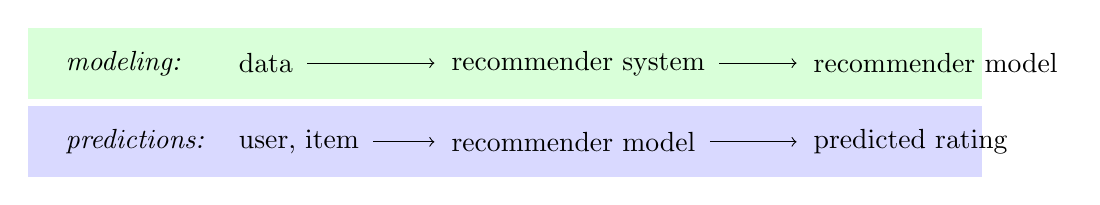
\begin{tikzpicture}[shorten >=1pt,->,draw=black, node distance=\layersep]

    \tikzstyle{every pin edge}=[<-,shorten <=2pt]
    \tikzstyle{rmodel}=[rectangle,fill=green!25,minimum size=20pt,inner sep=5pt]
    \tikzstyle{emodel}=[rectangle,fill=blue!25,minimum size=20pt,inner sep=5pt]
    \tikzstyle{amodel}=[rectangle,fill=red!25,minimum size=20pt,inner sep=5pt]
    \tikzstyle{blank}=[rectangle,right,fill=none,minimum size=20pt,inner sep=5pt]
      
    \fill[green!15] (0,1.1) rectangle (\textwidth,2);
    \fill[blue!15] (0,0.1) rectangle (\textwidth,1);
    
    \node[blank] (I2) at (0.3cm,  0.55) {\emph{predictions:}};
    \node[blank] (I1) at (0.3cm,  1.55)  {\emph{modeling:}};
    
    \node[blank] (I2) at (2.5cm, 0.55) {user, item};
    \node[blank] (I1) at (2.5cm, 1.55) {data};
   
    \node[blank] (P2) at (5.2cm, 0.55) {recommender model};
    \node[blank] (P1) at (5.2cm, 1.55) {recommender system};

    \node[blank] (O2) at (9.8cm, 0.55) {predicted rating};
    \node[blank] (O1) at (9.8cm, 1.55) {recommender model};
    
    \path (I1) edge (P1);
    \path (I2) edge (P2);

    \path (P1) edge (O1);
    \path (P2) edge (O2);
       
  \end{tikzpicture}

  \vspace{1em}
  \caption[Simplified Recommender System]{
    A simplified view of recommender systems:
    Ratings of items by users are used to create a \emph{model}.
    This model is then used to predict unknown ratings between users and items.
    Note that many recommender systems work differently,
    as we shall see later in this thesis.
  }
  \label{fig:simple-rs}
\end{figure}


Consider this: 
when an algorithm is selected for use in a recommender system,
there is a concious decision of which predictive data pattern to use.
Before any user modeling is performed, the researcher or developer selects
one or more methods that is thought to best model every user and item in the system.
While the methods themselves may perform well, their selection
reflects how whoever created the system assumes how each user
can and \emph{should} be modeled. This underlying subjectivity is not desirable.
We call this the \emph{latent subjectivity problem}.

Examples are not hard to come by.
For instance, while one user might appreciate social
influence in their search results, another user might not.
While one user might find frequency of communication maps well to relevance,
another might not. 
One user might feel the similarity of movie titles are a good predictor,
while another might be more influenced by production year.
Some users may favor items rated highly on a global scale,
while others are more interested in what users similar to themselves have to say.

The same problem exists for items. While one item might best be judged by its content,
another might be better described by previous ratings from other users.
One item's relevance may be closely tied to when it was created,
while other items may be timeless.
The exact differences are not important, only that they exist.

Another way to put this is that 
\emph{user modeling methods are dependent on the subjective assumptions of their creators}.
A modeling method use certain aspects of available data to make predictions,
and these aspects are chosen by whoever creates the system.

Modern aggregation approaches face the same problem. 
Aggregation is done on a generalized, global level,
where each user and item is expected to place the same importance on each modeling method.
While aggregation is selected to minimize some error over a testing set,
the subjective nature remains. The compiled aggregation is a generalization,
treating all users and items the same --- hardly a goal of user modeling.

Should it not be up to the users to implicitly decide which method best describes their preferences?
And, considering the vast scope of items we can come by, will the selected
methods really perform optimally for every item?
We believe the priority of each algorithm should be implicitly and automatically
based on how well they have previously worked for individual users and items.
Without this adaptability, it may be hard for recommender systems
to perform well in scenarios with widely differing users and items.
The scope of users and items is simply too great for any one or generalized combination
of methods to capture the nuanced nature of relevance prediction.

We propose a novel method that we call \emph{adaptive recommenders}, 
where the selection of algorithms is implicitly made by the users and items.
This provides an extra level of abstraction and personalization.
The selection decisions are implicit, and happens in the background, without any extra interaction required.
This leaves the subjective nature of selecting ways to model users and items where it should be.
That is, in the hands of individual users, and dependent on specific items.

This adaptive selection has an important consequence. 
If an algorithm is contextually used based on how well it performs,
any possibly useful recommender algorithm suddenly becomes a worthy addition.
Algorithms that perform well for a user or an item is selected for this task.
Those that do not will be used in other situations where they might be better suited.

As far as we know, such adaptive prediction aggregation has not been done before.
The main research question of this thesis is whether or not adaptive recommenders
can outperform traditional approaches.

\hr

\noindent
This thesis is structured as follows.
Chapter \ref{chap:theory} will present background theory and previous work for
the information overload problem, recommender systems, 
prediction aggregation (combining scores) and rank aggregation (combining sorted lists). 
We will also introduce briefly introduce the topics of information
retrieval and personalized search, which will serve
as a case study in later chapters.

Chapter \ref{chap:methods} will further discuss the latent subjectivity problem,
and build the \emph{adaptive recommenders} approach from the ground up.
We will show how this approach can be used for both prediction aggregation
and rank aggregation.

Chapter \ref{chap:results} will test three hypotheses and experiment with our newly built method.
We will experiment with prediction aggregating for singular items, and explore rank aggregation for personalized search.
Finally, Chapter \ref{chap:discussion} will discuss the implications of our results,
important limitations, contributions and suggest future work.



    \chapter{Background Theory}
      \section{User Modeling}

\emph{User Modeling (UM)} is about adapting an application to its users.
Whenever an application behaves or presents differently based on knowledge
of individual or groups of users, it is performing user modeling. 
Examples of UM include:

\begin{itemize*}
  \item Translating content based on user location.
  \item Suggesting interesting items based on previous activity.
  \item Reorganizing content based on predicted user relevance.
  \item Changing presentation to match user preferences or abilities.
  \item Any form of personalized content, presentation or behaviour from the application.
\end{itemize*}

Naturally, with such a vague definition, user modeling spans many fields,
approaches and methods. However, there are two core problems each method tries to solve:

\textbf{Information Overload} occurs when an application presents more information than a user is able to consume.
\cite{Bjorkoy2010d}
There are plenty of potential culprits: a poor signal to noise ratio, where relevant content is drowned out by useless 
information; an interface ill suited to the current user’s presentational needs or to the content being presented; 
a system that constrains the user, rather than adapt to how it is used. UM methods often apply personalization to solve this problem.
The thought is that a system that is personal, not general, will be better at tackling information overload.

\textbf{Content discovery} is closely related to information overload. As the amount of content increases,
finding and discovering relevant pieces of information becomes more difficult. Many UM methods
exists to automatically identify and present items based on knowledge of each user. For instance,
when a system allows explicit ratings of items, individually unseen and probably relevant items can be predicted
based on past user ratings.


There are two main approaches to user modeling, each led by a different field of computer science:

\emph{Artificial Intelligence (AI)} looks at user modeling from a bottom-up, computational perspective. 
The goal is to develop algorithms that reliably and effectively can create models of each user
and through these models predict future interaction or preferences. 

\emph{Human-Computer Interaction (HCI)} looks at user modeling from a top-down, interaction based perspective.
The goal here is to create approximate models of different stereotypical users to better understand how 
an application will be used. By examining the preferences, priorities and usage patterns of different groups
of users, the application can be adapted on a personal or stereotypical level.

This thesis takes the AI approach.

Problem statement

\begin{eqnarray}
  \mathrm{M_{UM}} = (I, C, U, F, u(i_i, c_u))\\
\end{eqnarray}

\subsection{Recommender Systems}

\begin{eqnarray}
  \mathrm{M_{RS}}   &=& (I, C, U, F,    u(i_i, c_u))\\
  \mathrm{M_{RSQ}}  &=& (I, C, Q, U, F, u(q_i, i_j, c_u))
\end{eqnarray}

Based on \cite[p2]{Adomavicius2005}.


\cite[p5]{Sugiyama2004} Example of collaborative recommendation: 
"Collaborative filtering can be represented as the problem of pre- dicting missing values in a user-item ratings matrix. Figure 3 shows a simplified example of a user-item ratings matrix.
In the neighborhood-based algorithm, a subset of users is first chosen based on their similarity to the active user, and a weighted combination of their rating is then used to produce predictions for the active user."

\cite[p2]{Bell2007b}: Sparsity, variety, numbers of ratings:
"First, the numbers of users and items may be very large, as in the Netflix data, with the former likely much larger than the latter.
Second, an overwhelming portion of the user-item matrix (e.g., 99\%) may be unknown. Sometimes we refer to matrix R as a sparse matrix, although its sparsity pattern is driven by containing many unknown values rather than the common case of having many zeros.
Third, the pattern of observed data may be very nonrandom, i.e., the amount of observed data may vary by several orders of magnitude among users or among items."

\cite[p2]{Bell2007b}: Shrinkage for parameter estimation:
"Although cross validation is a great tool for tuning a few param- eters, it is inadequate for dealing with massive numbers of param- eters. Cross validation works very well for determining whether the use of a given parameter improves predictions relative to other factors. However, that all-or-nothing choice does not scale up to se- lecting or fitting many parameters at once. Sometimes the amount of data available to fit different parameters will vary widely, per- haps by orders of magnitude. The idea behind “shrinkage” is to impose a penalty for those parameters that have less data associ- ated with them. The penalty is to shrink the parameter estimate towards a null value, often zero. "



\section{Personalized Search}

An Information Retrielal Model is a quadruple \citep[p23]{Baeza-Yates1999}:

\begin{eqnarray}
  \mathrm{M_{IR}} = (D, Q, F, r(q_i, d_i))
\end{eqnarray}

$D$ is the set of representations of the documents in the system. $Q$ is the set of logical user information needs, or queries.
$F$ is a framework for modeling documents, queries and their relationships.
$R(q_i, d_i)$ is a ranking function that associates a real number with a query and a document.
Such a ranking defines the ordering among documents with regard to query $q_i$.

Similar notation for FolkRank in \cite[p4]{Hotho}.

Conceptually, this is a graph.
Nodes, and F represents the edges.

\cite[p6]{Micarelli2007}: Three dimensions of user modeling in IR: Part of retrieval; re-ranking after
retrieval; query modification based on user model.

\begin{eqnarray}
  \mathrm{M_{PS}}  &=& (D, C, Q, U, F, R)\\
  \mathrm{R}       &=& (r(q_i, d_i), u(q_i, d_i, u_i))\\
  \mathrm{P_{c_i}} &=& (Q_{c_i}, U_{c_i}, F_{c_i})
\end{eqnarray}

$P_{c_i}$ is the user model. Model based. Create heuristic-based recommendations from this info.
(Explain conten/collaborative/hybrid and orthogonal model/heuristic based approaches).

IR can be seen as content-based RS. 
If we use a collaborative RS, get a 'pseudo-hybrid' solution. Not completely integrated,
but draws on both social connections and semantic relations.

Conceptually, this is still a graph.
Nodes, and F represents the edges.

Multiple models: Better than single algorithms. Two dimensions: 
1; Different scales of data (local/regional scale).
2; Multiple source of data with tailored algorithms.

Introduce pagerank, topic sensitive pagerank, personalized topic sensitive pagerank.

Trust of sites/other users can be one algorithm in an aggregate user model.

Feedback: 
\cite[p9]{Micarelli2007} implicit from usage data or explicit user profiles. 
\cite{Shen2005}: Use of imidiate previous search history to provide real-time updating of user models. Previous searches more important.

Modeling:
\cite{Jeh2003}: Partial personalized pagerank vector, to bias pagerank towards already visited or bookmarked sites.

\cite[p2]{Teevan2005a}: Implications of personalized search. Users have different needs/domains/expectations.
"The study suggests personalization of results via re-ranking would provide significant benefit for users."
"Importantly, there are still many relevant results at ranks 11-50, well beyond what users typically see. 
This suggests the search result ordering could be improved."
Standard sets give high correlation between user relevance judgements -- however, when asking users
to rank according to their personal expectations, the disparity increases rapidly. Weakness in 
traditional IR expert relevance judgement.

Google personalized Search: Give access to store search history, personalized results thereafter. See \url{google.com/psearch} [google psearch patent]; 
Google Alerts: Emails when new results on a query is available. See \url{http://www.google.com/alerts}.

\subsection{Tags in Personalized Search}

\cite[p4]{Noll2007}: 
Tagging can be interpreted as a relation R\_tagging < D * U * T, where D is the set of documents, U the set of users and T the set of tags.

\cite[p2]{Hotho}: Folksonomies as a ranking source: 
"To this end, we propose a formal model for folksonomies, and present a new algorithm, called FolkRank, that takes into account the folksonomy structure for rank- ing search requests in folksonomy based systems."
"The FolkRank ranking scheme has been used in this paper to generate personalized rankings of the items in a folksonomy, and to recommend users, tags and resources."

\cite{Dou2007}: Evaluation of personalized search with Rank Scoring and Average rank. 
Personalization strategies: Personal click score, user interest vectors (categories), 
group-level re-ranking. MSN query logs for testing. Click-personalization simple and stable, 
profile-based more unstable.

\cite[p2]{Teevan2005a}: Implications of personalized search. Users have different needs/domains/expectations.
"The study suggests personalization of results via re-ranking would provide significant benefit for users."
"Importantly, there are still many relevant results at ranks 11-50, well beyond what users typically see. 
This suggests the search result ordering could be improved."
Standard sets give high correlation between user relevance judgements -- however, when asking users
to rank according to their personal expectations, the disparity increases rapidly. Weakness in 
traditional IR expert relevance judgement.




\section{Aggregate Modeling}

Use simple algorithms over complex, monolithic ones. E.g., one algorithm can measure freshness - 0 when the rating is out of date, and 1 when it's completely fresh.




    \chapter{Methods \emph{\&} Implementation}
      \label{chap:methods}

In this chapter, we will build our approach to user modeling.
We will first explain why a new approach is needed,
and develop three hypotheses based on the 
assumptions in Chapter \ref{chap:intro}.
The two final sections will show how \emph{stacked recommenders}
can perform prediction aggregation in a recommendation scenario,
and rank aggregation in a personalized search scenario.

\section{Latent Subjectivity}
\label{sec:reasoning}

As described in the previous chapter, 
there are many ways of predicting the
relevance of an item to a user. 
In fact, judging by the number of different approaches,
the only limiting factor seems to be the different 
patterns researchers discover in available data.

As described in Section \ref{sec:aggregate},
modern approaches to recommender systems try to combine many of these methods.
By leveraging so called \emph{disjoint patterns}
in the data, several less than optimal predictors
can be combined, so that the combination outperforms the individual algorithms.
Moderns search engines work much in the same way,
combining multiple ranking signals into a final results list
(see Section \ref{subsec:signals}).

Why then, when we have all these valid approaches, would we need yet another technique?
As explained in Chapter \ref{chap:intro}, 
we believe the \emph{latent subjectivity problem}
is a fundamental issue with each approach described so far.
Consider the following examples of relevance judgement:

\begin{itemize*}
  \item PageRank \citep{Bender2005} assumes that the relevance of a web page is 
  represented by its authority, as computed from inbound links from other sites.
  \item Some systems considers a user's social connections to be important
  in ranking search results, when performing personalized search (e.g. \cite{Carmel2009}).
  \item When recommending movies, one predictor may be based on the ratings
  of users with similar profile details. Another predictor might be 
  dependent on some feature, e.g. production year of well liked movies.
  \item SVD-based approaches assume global patterns and groups of users and items
  are best suited to produce predictions (see Section \ref{subsec:recommender:examples}).
  \item Recommendations based on the Pearson Correlation Coefficient \cite[p.11]{Segaran2007}
  assumes that the statistical correlation between user ratings is a good
  measure for user similarity.
\end{itemize*}

While these methods may perform well, their selection
reflects how whoever created the system assumes how users
can and \emph{should} be modeled. This underlying subjectivity is not desirable.
We see two different approaches one can take when creating a recommender system,
represented by two questions:

\clearpage

\begin{enumerate*}
  \item What combination of which methods will accurately predict unknown scores?
  \item Which methods could possibly help predict a score for a user or an item?
\end{enumerate*}

The first question is what has to be considered in traditional modeling aggregation.
First, a set of applicable methods leveraging disjoint patterns must be selected. 
Then, an optimal and generalized combination of these must be found,
most often through minimizing the average error across all users.

The second question is quite different. 
Instead of looking for an optimal set of methods and an optimal combination,
we look for the set of \emph{any applicable methods} that \emph{some users} might find helpful,
or that might work for \emph{some items}.
We believe this is a much simpler problem. 
Instead of trying to generalize individuality,
it can be embraced, by allowing users to implicitly and automatically select which methods they prefer,
from a large set of possible predictors.

As explained in Chapter \ref{chap:intro}, 
assuming that users will place similar importance on each modeling method is 
contrary to the goals of user modeling. 
Our goal should instead be a system which can leverage the differences
between users and employ the available algorithms based on their individual preferences.

Just as users are different, items have their own characteristics.
Needless to say, items are often quite different from another,
along a myriad of dimensions. For example,
if items correspond to websites, the number of metrics we can use to judge
the relevance of an item is immense.
If items are indeed as different as the users themselves, it stands to reason that the same 
modeling method will not perform as well for every item.

An approach where we only need to consider the second question is desirable.
Regardless, both traditional, single-approach modeling methods, and modern aggregation approaches
often treat every user and item the same. No matter its intrinsic qualities, an element will be judged
by the same methods as every other element. 

This chapter will develop a way to aggregate a host of modeling methods on a per-user and per-item basis.
By adapting the aggregation to the current item and user, we should be able to mitigate the latent subjectivity problem. 
This adaptive aggregation is performed implicitly and automatically,
without any extra interaction required from each user.

As mentioned in Chapter \ref{chap:intro}, this has an important consequence.
If each algorithm is \emph{only used} in situations it will probably perform well,
any possible recommender algorithm becomes a worthy addition.
In other words, instead of finding an optimal combination,
we can use any algorithm that \emph{might work for some elements}
in our aggregation.

With adaptive recommenders, the users are in control of which methods best fit their needs, and
a method's priority is influenced by how well it performs for the current item.
However, in order to test whether or not these assumptions hold,
we need a set of testable hypotheses.

\clearpage

\section{Hypotheses}

So far we have taken a look at approaches to recommendations and personalized search:
Traditionally, a single method that considers some pattern in the data is used.
Modern techniques blend different methods to achieve a combined accuracy 
that outranks the performance of each individual method.

However, based on the notion of latent subjectivity in method selection and aggregation,
we desire an even more personalized technique. 
To this end, this paper will test three hypotheses (H1-H3), in an effort to establish
whether per-user aggregation is a viable technique. First:

{
  \itshape
  $\mathbf{H1}$: The accuracy of user-item relevance predictions can be improved
  by blending multiple modeling methods on a per-user basis:
  $\forall m \in M: \mathrm{error}(am_u) < \mathrm{error}(m)$.
}

It stands to reason that if a recommender system is indeed impaired
by the subjective selections of modeling methods,
a per-user blend of these methods should outperform each of the individual approaches.
Second:

{
  \itshape
  $\mathbf{H2}$: A per-user aggregation method can outperform global and generalized 
  blending methods:
  $\forall a \in A: \mathrm{errorr}(am_u) < \mathrm{error}(a)$.
}

If our assumption that model aggregation inherits the subjective nature of its chosen parts,
a per-user aggregation without such misplaced subjectivity should outperform a
generalized blending.
Third:

{
  \itshape
  $\mathbf{H3}$: The result set from an information retrieval query
  can be personalized by blending multiple modeling methods on a per-user basis.
}

As described in Section \ref{subsec:signals},
every measure that influence the final ranking of results from a search engine
can be seen as individual signals. Each signal, be it an IR score,
something like PageRank or the result of a user modeling method,
contributes to the final ranking.
As the aggregation of these signals are the same problem faced
when aggregating recommender systems,
a per-user approach to blending signals should be able to
produce a set of personalized search results.
In other words, techniques from information retrieval and user modeling
should be combined on a per-user basis to provide individually adapted results.


\section{Adaptive Recommenders}
\label{sec:usermetamodeling}

\emph{Adaptive Recommenders} (AR) is a technique for combining many recommender systems
in a way that is optimal for the each user and each item.
Given that we wish to predict the relevance of an item to a user,
using many methods that consider disjoint data patterns,
we have two important questions:

\begin{enumerate*}
  \item What rating does each method predict?
  \item How accurate will each of these predictions be?
\end{enumerate*}

Recommender systems traditionally only care about the first question:
a single method is used to predict an unknown rating.
Modern aggregation techniques goes one step further, and combines many methods using a generic (often weighted) combination.
We wish to make the aggregation \emph{adaptive},
so that the aggregation itself depends on which user and which item we are considering.

Formally, we define adaptive recommenders as \emph{adapting a set of recommender systems
with another complementary set of recommender systems} 
(see Figure \ref{fig:adaptiveusermodeling}).
This then is a form of meta-modeling, where one set of modeling methods is adapted by another set of modeling methods.
The first set creates standard prediction scores, and answers the first question.
The second set predicts how accurate each method will be for the current user and item,
answering the second question.
The interesting bit is that AR can use recommender systems for both these tasks, as we shall see.
A system for adaptive recommenders is specified by a 6-tuple:

\begin{eqnarray*}
  \mathrm{AR} &=& (Items, Users, Ratings, Framework, Methods, Adapters)\\
              &=& (I,U,R,F,M,A).
\end{eqnarray*}
%
We have sets of $Users$ and $Items$, and a set of $Ratings$.
Each user $u \in U$ can produce a rating $r \in R$ of an item $i \in I$.
As mentioned, items can be just about anything, for example documents, websites, movies, events, or indeed, other users.
The ratings can be explicitly provided by users, for example by rating movies,
or they can be mined from existing data, for example by mining query logs.
As before, we use the term \emph{rating} loosely --- equivalent terms include \emph{relevance}, \emph{utility},
\emph{score} or \emph{connection strength}. In other words, this is a measure of what a user thinks of an item
in the current domain language. However, since \emph{rating} will match the case study we present in the next chapter,
we will be using this term. 

\begin{figure}[t]
  \centering 
  \begin{minipage}{0.49\textwidth}
    \centering 

    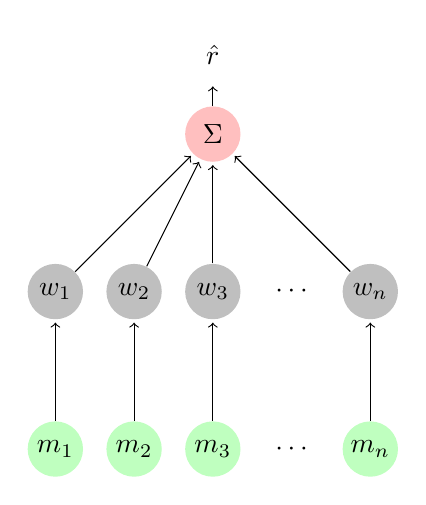
\begin{tikzpicture}[shorten >=1pt,->,draw=black, node distance=\layersep]
      \tikzstyle{every pin edge}=[<-,shorten <=2pt]
      \tikzstyle{node}=[circle,fill=black!25,minimum size=20pt,inner sep=0pt];
      \tikzstyle{method}=[node,fill=green!25];
      \tikzstyle{weight}=[node,fill=black!25];
      \tikzstyle{error}=[node,fill=blue!25];
      \tikzstyle{agg}=[node,fill=red!25];
      \tikzstyle{txt}=[node,fill=white];
       
      \node[method] (M1) at (0,-6) {$m_1$};      
      \node[method] (M2) at (1,-6) {$m_2$};         
      \node[method] (M3) at (2,-6) {$m_3$};         
      \node[txt]    (MS) at (3,-6) {$\cdots$}; 
      \node[method] (MN) at (4,-6) {$m_n$};
      \node[weight] (W1) at (0,-4) {$w_1$};      
      \node[weight] (W2) at (1,-4) {$w_2$};         
      \node[weight] (W3) at (2,-4) {$w_3$};         
      \node[txt]    (WS) at (3,-4) {$\cdots$}; 
      \node[weight] (WN) at (4,-4) {$w_n$};
      \node[agg]    (AG) at (2,-2) {$\Sigma$};
      \node[txt]    (RS) at (2,-1)  {$\hat{r}$};
      
      \path (M1) edge (W1);
      \path (M2) edge (W2);
      \path (M3) edge (W3);
      \path (MN) edge (WN);
      \path (W1) edge (AG);
      \path (W2) edge (AG);
      \path (W3) edge (AG);
      \path (WN) edge (AG);
      \path (AG) edge (RS);
    \end{tikzpicture}
  \end{minipage} 
  \hfill 
  \begin{minipage}{0.49\textwidth}
    \centering 

    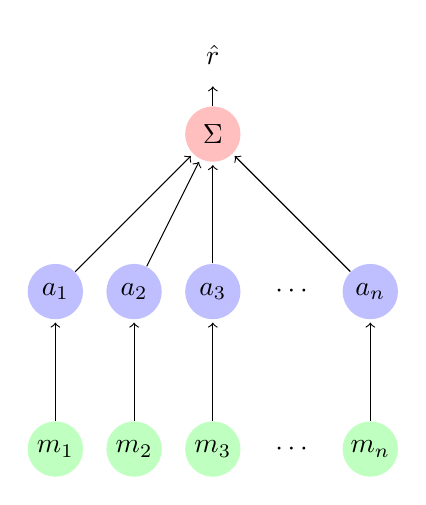
\begin{tikzpicture}[shorten >=1pt,->,draw=black, node distance=\layersep]
      \tikzstyle{every pin edge}=[<-,shorten <=2pt]
      \tikzstyle{node}=[circle,fill=black!25,minimum size=20pt,inner sep=0pt];
      \tikzstyle{method}=[node,fill=green!25];
      \tikzstyle{weight}=[node,fill=black!25];
      \tikzstyle{error}=[node,fill=blue!25];
      \tikzstyle{agg}=[node,fill=red!25];
      \tikzstyle{txt}=[node,fill=white];
       
      \node[method] (M1) at (0,-6) {$m_1$};      
      \node[method] (M2) at (1,-6) {$m_2$};         
      \node[method] (M3) at (2,-6) {$m_3$};         
      \node[txt]    (MS) at (3,-6) {$\cdots$}; 
      \node[method] (MN) at (4,-6) {$m_n$};
      \node[error]  (E1) at (0,-4) {$a_1$};      
      \node[error]  (E2) at (1,-4) {$a_2$};         
      \node[error]  (E3) at (2,-4) {$a_3$};         
      \node[txt]    (ES) at (3,-4) {$\cdots$}; 
      \node[error]  (EN) at (4,-4) {$a_n$};
      \node[agg]    (AG) at (2,-2) {$\Sigma$};
      \node[txt]    (RS) at (2,-1)  {$\hat{r}$};
      
      \path (M1) edge (E1);
      \path (M2) edge (E2);
      \path (M3) edge (E3);
      \path (MN) edge (EN);
      \path (E1) edge (AG);
      \path (E2) edge (AG);
      \path (E3) edge (AG);
      \path (EN) edge (AG);
      \path (AG) edge (RS);
    \end{tikzpicture}
  \end{minipage} 
  \vspace{2em}
  \caption[Comparison of Aggregation and Adaption]{
    Comparison of aggregation and adaption:
    (left) modern aggregation approaches uses a set of pretrained weights
    to prioritize each modeling method.
    The weighted predictions are aggregated into a final prediction $\hat{r}$.
    (right) Adaptive user modeling employs secondary modeling methods instead
    of weights. These estimate the accuracy of the initial method
    for the current user and item.
  }
  \label{fig:layer:comparison}
\end{figure}




The $Framework$ variable specifies how the data is represented.
The two canonical ways of representing users, items and ratings are graphs and matrices (see Section \ref{sec:recommender}).
We shall use a matrix, where the first dimension corresponds to users, the second to items, and each populated cell is an explicit or implicit rating:

\begin{eqsp}
 R_{u,i} =
 \begin{pmatrix}
  r_{1,1} & r_{1,2} & \cdots & r_{1,i} \\
  r_{2,1} & r_{2,2} & \cdots & r_{2,i} \\
  \vdots  & \vdots  & \ddots & \vdots  \\
  r_{u,1} & r_{u,2} & \cdots & r_{u,i}
 \end{pmatrix}.
\end{eqsp}
%
As we wish to leverage disjoint data patterns, we have a set of modeling $Methods$, 
each with their own way of estimating unknown ratings. 
Each model $m \in M$ is used to compute independent and hopefully complimentary predictions.
In our case, these methods are recommender systems.

As demonstrated in Chapter \ref{chap:theory}, there are many different recommendation algorithms,
that consider different aspects in the data, for example users, items and ratings, as well as 
sources such as intra-user connections in social networks or intra-item connections in information retrieval systems.
Examples of such recommender systems include Slope One predictions, SVD factorization and Nearest Neighbor weighted predictions
(see Section \ref{subsec:recommender:examples}).
These methods predict unknown connections between users and items based on some pattern in the data,
for example user profile similarity, rating correlations or social connections.
As previously explained, to achieve the best possible combined result, we wish to use methods that look at disjoint patterns, 
i.e. complementary predictive parts of the data (see Section \ref{sec:aggregate}).

The $Adapters$ part of our 6-tuple refers to the second level of user modeling methods.
In traditional prediction aggregation this is a simple linear function for combining the different predictions,
for example by pre-computing a set of weights, one for each method.
As found by \citet[p6]{Bell2007} the accuracy of the combined predictor is more dependent on the 
ability of the various predictors to expose different aspects of the data, than on 
the individual accuracy of each predictor.
As described in Section \ref{sec:aggregate}, multiple prediction results are normally 
combined into a final singular result,
based on a generalized combination found by minimizing some error across all users.

With adaptive recommenders, the $Adapters$ are themselves user modeling methods 
(see Figure \ref{fig:layer:comparison}).
However, instead of modeling users, we wish to model each recommender system.
More specifically, we wish to model the \emph{accuracy} of each recommender system.
Methods in this second layer are used to predict how accurate each of their corresponding basic recommenders will be.
It is these methods that will allow us to do adaptive aggregation based on the current user and item.
We then have two distinct layers of user modeling 
(see Figure \ref{fig:adaptiveusermodeling}):

\begin{figure}
  \center
  \def\layersep{1.8cm}
  \begin{tikzpicture}[shorten >=1pt,->,draw=black, node distance=\layersep]

    \tikzstyle{every pin edge}=[<-,shorten <=2pt]
    \tikzstyle{node}=[circle,fill=black!25,minimum size=20pt,inner sep=0pt]
    \tikzstyle{input node}=[node, fill=green!25];
    \tikzstyle{output node}=[node, fill=red!25];
    \tikzstyle{hidden node}=[node, fill=blue!25];
    \tikzstyle{annot} = [text width=10em, text centered]
    \tikzstyle{txt}=[node,fill=white];
    
    \node[txt] (UI) at (0,-2) {$(u,i)$};  

    \node[input node] (I-1) at (\layersep,-1) {$m_1$};
    \node[txt]        (I-D) at (\layersep,-2) {$\vdots$};
    \node[input node] (I-N) at (\layersep,-3) {$m_n$};
    
    \node[txt] (P-1) at (\layersep*2, -1) {$p_1$};
    \node[txt] (P-D) at (\layersep*2, -2) {$\vdots$};
    \node[txt] (P-N) at (\layersep*2, -3) {$p_n$};

    \node[hidden node] (H-1) at (\layersep*3, -1) {$a_1$};    
    \node[txt]         (H-D) at (\layersep*3, -2) {$\vdots$};    
    \node[hidden node] (H-N) at (\layersep*3, -3) {$a_n$};    

    \node[txt] (R-1) at (\layersep*4, -1) {$(p_1,w_1)$};
    \node[txt] (R-D) at (\layersep*4, -2) {$\vdots$};
    \node[txt] (R-N) at (\layersep*4, -3) {$(p_n,w_n)$};
    
    % hidden helper node
    \node[txt] (HH)  at (\layersep*5,-1) {};

    % Draw the output layer node
    \node[output node,pin={[pin edge={->}]right:$\hat{r}$}] at (\layersep*5,-2) (O) {$\Sigma$};
    
    \path (UI) edge (I-1);
    \path (UI) edge (I-N);

    \path (I-1) edge (P-1);
    \path (I-N) edge (P-N);

    \path (P-1) edge (H-1);
    \path (P-N) edge (H-N);

    \path (H-1) edge (R-1);
    \path (H-N) edge (R-N);

    \path (R-1) edge (O);
    \path (R-N) edge (O);

    % Annotate the layers
    \node[annot,above of=I-1, node distance=1cm] {\emph{prediction}};
    \node[annot,above of=H-1, node distance=1cm] {\emph{adaption}};
    \node[annot,above of=HH,  node distance=1cm] {\emph{aggregation}};
  \end{tikzpicture}

  \vspace{1em}
  \caption[The Layers of Recommenders]{
    Layers of recommenders. 
  }
  \label{fig:adaptiveusermodeling}
\end{figure}


\begin{enumerate}
  \item
    \emph{The methods layer} consists of traditional user modeling methods, that use a single aspect of the data to produce predictions.
    When presented with an item and a user, these methods produce a predicted rating $\hat{r}_{u,i}$ based on their algorithms.
  \item
    \emph{The adaptive layer} is another set of corresponding modeling methods, that work a bit differently.
    These methods take an item and a user and estimates how well its underlying method will perform this prediction.
    The accuracy estimations are then combined with the predictions by aggregation.
    Each of these adaptive methods do not have to employ the same algorithm as their corresponding methods,
    the layers are only similar in that both consist of recommender systems.
\end{enumerate}

Another way of describing (and implementing) these two levels is through 
the $\mathrm{map}$ and $\mathrm{reduce}$ functions of functional programming.
For example, we can express prediction aggregation as 

\begin{eqsp}
  \hat{r}_{u,i} = \mathrm{reduce}(u, i, \mathrm{map}(M, u, i)).
\end{eqsp}
%
First, each modeling method is applied by the $\mathrm{map}$ function, with the current user, item and set of modeling methods as input.
This operation returns a set of scalar prediction values. 
These values are then combined by the $\mathrm{reduce}$ function, which also takes the current user and item as input.
In our terms, $\mathrm{map}$ is the methods layer, and $\mathrm{reduce}$ is the adaptive layer.
If we wish to do rank aggregation, the equation is a bit different:

\begin{eqsp}
  \tau_{u,n} = \mathrm{reduce}(u, \mathrm{map}(M,u,n)).
\end{eqsp}
%
Here, $\tau_{u}$ is the list of recommended items for user $u$ (following the notation in \citet[p3]{Dwork2001}).
Note that there is no input item in this formula as we wish to produce a ranking of the top $n$ recommended items.
The result is an adaptively sorted list of the top $n$ items for the current user.
A common use case for rank aggregation is personalized search:
an IR algorithm restricts the item space, which is then adapted by recommender systems,
as we shall see.

Expressing ourselves in terms of $\mathrm{map}$ and $\mathrm{reduce}$ is helpful 
as this will guide our implementation.
Note that our terminology is a bit different from the proper MapReduce framework
for parallel computation (as explained in \citet[p75]{Manning2008}).
However, as with the standard key/value approach to MapReduce,
the fact that our tasks can be run in parallel will help
us implement efficient algorithms.


\subsection{Adaptive Aggregation}

To perform adaptive recommender aggregation, we need the $Adapters$ to be actual recommender systems.
Until now we have talked about both prediction aggregation (scores) and rank aggregation (sorted lists).
For now we shall stick to scalar predictions, but will return to rank aggregation in Section \ref{sec:methods:rank}.

The simplest generalized way of prediction aggregation is to take the average of all predictions made
by the different methods (e.g. \citet[p3]{Aslam2001}):

\begin{eqsp}
  \hat{r}_{u,i} = \frac{1}{N} \sum_{m \in M} p(m,u,i).
\end{eqsp}
%
Here, $\hat{r}_{u,i}$ is the estimated rating from user $u$ to item $i$,
$N$ is the number of methods in $M$, and $p(m,u,i)$ is the predicted rating from method $m$.
To achieve an even more optimal result, 
many aggregators weigh each method differently (e.g. \cite{Claypool1999}):

\begin{eqsp}
  \hat{r}_{u,i} = \sum_{m \in M} w_{m} \times p(m,u,i) 
  \quad \text{where} \quad 0 \leq w_{m} \leq 1, \quad \sum_{m \in M} (w_m) = 1.
\end{eqsp}
%
In this equation, $w_m$ is the weight applied to modeling method $m$. 
These weights fall in the range $[0,1]$ and sum up to $1$.
As described in \ref{sec:aggregate}, 
these weights can be estimated by different machine learning methods.
However, as discussed in Section \ref{sec:reasoning},
this is still a generalized result, averaged across every user and item.
The system assumes that the best average result is the best result for each individual user and item.
This means that, even with method-specific weights, we are still hindered by the latent subjectivity problem.

In order to leverage as many patterns as possible while sidestepping any latent subjectivity,
we need \emph{adaptive weights} that are computed specifically for each combination of a user and an item.
This is more difficult than simply estimating generalized weights.
If we wish each weight to be combination-specific, then pre-computing each weight for each method becomes unfeasible.
We would have to compute a weight for each method for each possible rating.
The adaptive weights also have to be estimated just as the unknown ratings:

\begin{eqsp}
  \hat{r}_{u,i} = \sum_{m \in M} p_{w}(m,u,i) \times p_{r}(m,u,i)
  \quad \text{where} \quad
  \sum_{m \in M} (p_{w}(m,u,i)) = 1.
\end{eqsp}
%
Here, $p_w(m,u,i)$ is the predicted optimal weight for method $m$ when applied to user $u$ and item $i$.
Adaptive recommenders is one way to estimating these weights, i.e. one way to implement $p_w$.

We wish to use standard recommender systems for predicting optimal adaptive weights.
To do this, we need to create a matrix (or graph)
that stores known values of how accurate some of the rating predictions will be.

The key insight is that \emph{the predicted accuracy of a method is the opposite of its predicted error}.
By modeling the errors of a method through standard recommender systems,
we can in turn predict errors for untested combinations
(see Figure \ref{fig:adaptiveweights}).
If we predict the error of a recommender system for a user and an item,
we have also predicted its accuracy.
To achieve this, we create an \emph{error matrix}:

\begin{figure}[t]
  \center
  \def\layersep{3cm}
  \begin{tikzpicture}[shorten >=1pt,->,draw=black, node distance=\layersep]

    \tikzstyle{every pin edge}=[<-,shorten <=2pt]
    \tikzstyle{rmodel}=[rectangle,fill=green!25,minimum size=20pt,inner sep=5pt]
    \tikzstyle{emodel}=[rectangle,fill=blue!25,minimum size=20pt,inner sep=5pt]
    \tikzstyle{amodel}=[rectangle,fill=red!25,minimum size=20pt,inner sep=5pt]
    \tikzstyle{blank}=[rectangle,fill=white,minimum size=20pt,inner sep=5pt]
    
    \node[blank] (UI) at (0,-0.5) {(u,i)}; 

    \node[blank] (EM) at (\layersep,-1) {error model};
    \node[blank] (RM) at (\layersep,0) {ratings model};
    
    \node[blank] (ER) at (\layersep*2,-1) {predicted error};
    \node[blank] (RR) at (\layersep*2,0) {predicted rating};
 
    \node[blank] (AG) at (\layersep*3,-0.5) {adaption};
    \node[blank] (W) at (\layersep*3.5,-0.5) {$\hat{pr}$}; 
    
    \path (UI) edge (EM);
    \path (UI) edge (RM);
    \path (EM) edge (ER);
    \path (RM) edge (RR);
    \path (ER) edge (AG);
    \path (RR) edge (AG);
    \path (AG) edge (W);
       
  \end{tikzpicture}

  \vspace{1em}
  \caption[Multiple Models for Adaptive Weights]{
    Multiple models for adaptive weights: 
    The data flow through the adaption of a single recommender method.
    The current user and item is fed into two distinct models: the ratings model, which 
    predicts unknown ratings, and the error model, which predicts how accurate 
    this rating will be for the current input. 
    The two predictions are then aggregated into a final part of a rating ($\hat{pr}$).
    Each of the recommender stacks contribute parts to the final rating.
  }
  \label{fig:adaptiveweights}
\end{figure}


\begin{eqsp}
 E_{u,i} =
 \begin{pmatrix}
    e_{1,1} & e_{1,2} & \cdots & e_{1,i} \\
    e_{2,1} & e_{2,2} & \cdots & e_{2,i} \\
    \vdots  & \vdots  & \ddots & \vdots  \\
    e_{u,1} & e_{u,2} & \cdots & e_{u,i}
 \end{pmatrix}
\end{eqsp}
%
Creating an error matrix for each modeling method is done by splitting the ratings data in two.
The first set can be used for the actual RS modeling, and the second
can be used to populate an error matrix for each RS.

With adaptive recommenders, each standard modeling method produces an error matrix where some of the cells have values.
A value in this matrix corresponds to the prediction error for a combination of a user and an item.
To achieve this, each modeling method is only trained with a part of the ratings data.
The error matrix is populated from the rest of the data,
by computing the error of each known rating the method was not trained for:

\begin{eqsp}
  \forall (u,i,r) \in (d_e - d_m): E(m)_{u,i} = |r - p(m,u,i)|
  \quad
  \text{where}
  \quad
  d_e,d_m \subset D
\end{eqsp}
%
Here, $D$ is the current dataset, and
$d_m$ and $d_e$ are subsets of $D$.
$m$ is a modeling method trained with the subset $d_m$.
To populate the error matrix for this method,
we take each rating which have not been used to train the method
and calculate the error of the method on this combination.
Since we are only interested in the magnitude of each error,
we take the absolute value of each measurement.
The result is a sparse error matrix we can use to predict unknown errors.

Notice the similarity of this matrix and the previously introduced ratings matrix.
This similarity is what will allow standard recommender systems
to perform adaptive aggregation.
Whenever we wish to train a new modeling method,
we apply the following algorithm:

\begin{enumerate*}
  \item Split the ratings data into two sets for training and error estimation.
  \item Train the modeling method in its specific way with the first training set.
  \item Use the error estimation data set to create the error matrix.
  \item Train an error model based on the error matrix.
\end{enumerate*}

The error models are trained using standard recommender systems.
After all, the expected input and output is the same.
We have two dimensions, with a sparse set of known connections,
and wish to predict unknown connections from this data.
The result is a set of modeling methods
that can predict the error of a recommender system
when its used on a particular user and item combination.

What will happen when we train a recommender system with the error matrix?
First of all, the errors will be on the same scale as the initial ratings.
Second, just as the ratings matrix will include noise (ratings that
do not contribute to any underlying pattern), this will be 
true for the error matrix as well.

For example, one method might have a large error for a particular user and item combination,
yet still work well for both these elements. 
However, this is just the kind of noise recommender systems are good at pruning away.
What we are interested in are situations where a method
has stable and significant errors for many ratings from a user,
or many ratings of an item.
In this case, there is a pattern where this method does not 
work well for the element in question.
This is exactly the kind of pattern recommender systems are good at identifying.

The same capabilities that makes recommender systems work well
on the ratings matrix, will also make them work well on the error matrix.
The properties we need for predicting ratings
are the same as those needed to predict accuracy.

Of course, some recommender systems will work better than others for the adaptive layer.
Most often we are seeking global patterns in the data.
We are looking for groups of users or items (or both) that suite some 
recommenders especially well, or that some recommenders will not work for.
SVD-based recommenders is one type of RS that can be used for this purpose.
By reducing the method-error space into an \emph{error category space},
we can identify how well a set of groups suite each available method.
We will get back to this when performing experiments in the next chapter.

When we have an error model for each modeling method, 
we can use these errors to estimate each weight.
Whenever we wish to create an adaptive aggregate prediction,
we apply the following algorithm:

\begin{enumerate*}
  \item Collect predictions from each modeling method for $(u,i)$.
  \item Collect estimated errors for each method for $(u,i)$.
  \item Compute weights for each method based on their relative predicted errors.
  \item Sum the weighted predictions to get the adaptively predicted rating.
\end{enumerate*}

The next section will explain these steps in detail.
We can now express the prediction phase of adaptive recommenders as an equation.
Each rating/relevance prediction is weighted by its predicted accuracy,
conditioned on the current user and item:

\begin{eqsp}
  \hat{r}_{u,i} = \sum_{(m_{e}, m_{r}) \in M} (1 - 
  \frac{
    p(m_{e},u,i)
  }{
    error(u,i)
  }) \times p(m_{r},u,i)
  \quad
  \text{where}
  \quad
  error(u,i) = \sum_{m_e \in M} p(m_e,u,i) 
\end{eqsp}
%
In this equation, each recommender method has two corresponding models:
$m_r$ is the ratings model, used to predict ratings, and
$m_e$ is the error model, used to predict errors.
$p(m,u,i)$ is the prediction of the model $m$ (a recommender system)
for the relevance of item $i$ to user $u$.
Each method is weighted by its predicted accuracy.
The weights are computed by taking the opposite
of each methods predicted error.
The errors are normalized across each user and item by $errors(u,i)$,
which is the sum of the errors of each method for the current combination.
This gives us weights in the range $[0,1]$ ensuring
final rating predictions on the same scale as that returned by the basic recommenders.

%For now, we have our approach to adaptive recommenders:
%
%\begin{eqsp}
%  \hat{r}_{u,i} = \sum_{(m_{e}, m_{r}) \in M} (1 - p(m_{e},u,i)) \times p(m_{r},u,i),
%\end{eqsp}
%
%where $p$ returns a prediction from a model for a specific user and item,
%$m_{r}$ is a standard recommender model, 
%and $m_{e}$ is its corresponding error model.
%For this equation to work as expected, the weights must be normalized:
%
%\begin{eqsp}
%  0 \leq p(m_e,u,i) \leq 1 \quad \text{and} \quad \sum_{m \in M} (p(m_e,u,i)) = 1.
%\end{eqsp}

Notice that the \emph{only} difference between $m_e$ and $m_r$ is how they are created.
$m_r$ is trained with the standard ratings matrix, and $m_e$ is trained using the error matrix.
This means we can use \emph{any} standard recommender system to perform adaptive aggregation.
Hence, the name \emph{adaptive recommenders}:
a set of secondary recommenders is used to adapt a set of standard
recommenders to each user and item.

It is also important to note that the types of recommenders used for the adaptive layer
is independent of the basic recommenders.
Each adaptive recommender need only predicted ratings from each basic recommender,
and does not care which algorithm it employs.
When making predictions, the calculations in the methods layer and adaptive layer
are independent of each other, as both use pre-computed models:
the method layer use the ratings matrix, or their own models
created during training, while the adaptive layers use the error matrices for each
basic method.

The result of this is a system that does not only aggregate a number of predictions for each unknown
combination of users and items,
but that also combines these methods based on how accurate each prediction is likely to be.

Let us now see how adaptive recommenders may be implemented.
We shall first do prediction aggregation in a recommendation scenario,
then rank aggregation in an information retrieval scenario.


\section{Prediction Aggregation}

Adaptive prediction aggregation means combining the results
from multiple scalar predictors conditioned on the current context.
As mentioned, we have two levels of predictors.
The first level is a set of traditional recommender systems
that produce estimations of unknown ratings between users and items.
The second level is another set of recommender systems 
that predict how accurate each of the first level recommenders will be.
There are two distinct phases when using adaptive recommenders:

\begin{enumerate*}
  \item The modeling phase creates the user models for both levels.
  \item The prediction phase uses the created models to estimate ratings.
\end{enumerate*}

We shall first explain the modeling phase, then the prediction phase.
The next section will explain a similar situation where
we wish to do \emph{adaptive rank aggregation} by 
combining ordered lists of results, depending on the current user and item.


\subsection{Modeling Phase}

Listing \ref{code:training} gives the basic algorithm for training
our models. The input to this method is the standard ratings matrix,
and a set of untrained modeling methods (in this case,
untrained recommender systems).

\begin{algorithm}
  \begin{algorithmic}[1]
  \REQUIRE ratings: The ratings matrix
  \REQUIRE methods: The set of modeling methods
  \ENSURE  rating\_models, error\_models: trained rating and error models 
    \STATE $rating\_models \gets \emptyset$
    \STATE $error\_models \gets \emptyset$
    \FORALL{$m \in methods$}
      \STATE $sample \gets \mathrm{BootstrapSample}(ratings)$
      \STATE $rating\_models_m \gets \mathrm{TrainModel}(m, sample)$
      \STATE $error\_models_m  \gets \mathrm{TrainErrorModel}(rating\_models_m, ratings)$
    \ENDFOR 
  \RETURN $(rating\_models, error\_models)$
  \end{algorithmic}
  \caption[Adaptive Prediction Aggregation Modeling]{Adaptive Prediction Aggregation Modeling
  }
  \label{code:training}
\end{algorithm}

An important question is how we should split the ratings data.
In this scenario, we need to split the data for a number of purposes.
The following sets must be created during training:

\begin{enumerate*}
  \item Training sets for the standard recommenders.
  \item Training sets for the error estimation models.
  \item A testing set to measure the performance of our final system.
\end{enumerate*}

Constructing these subsets of the available data is a common task in ensemble learning
\cite[p.7]{Polikar2006}.
As seen in Listing \ref{code:training}, we use an approach called 
\emph{bootstrap aggregation}, also known as \emph{bagging}
(introduced by \cite{Breiman1996}).
Originally, bagging is used by ensemble learning classification methods, where multiple classifiers are 
trained by uniformly sampling a subset of the available training data. 
Each model is then trained on one of these subsets, and the models are aggregated by averaging their individual predictions.

Formally, given a training set $D$ with $n$ items, bagging creates $m$ new training sets of size $n' \leq n$ by sampling
items from $D$ uniformly and with replacement. 
In statistics, these types of samples are called \emph{bootstrap samples}.
If $n'$ is comparable in size to $n$, there will be some items
that are repeated in the new training sets.

Bagging suits our needs for a few reasons. First, it helps create disjoint predictors, 
since the predictors are only trained (or specialized for) a subset of the available data.
When using multiple similar recommenders, this means we can create specialized models
for parts of the data with a higher performance than if they were trained on the entire dataset.
Second, bagging allows us to easily train the underlying modeling methods without any complex partitioning of the data.
To partition and use the available data, we use the following algorithm:

\begin{enumerate*}
  \item Split the entire dataset into a training and testing set.
  \item Train modeling methods through bootstrap aggregation of the training set.
  \item Train error models from the complete training set.
  \item Test the resulting system with the initial testing set.
\end{enumerate*}

Each modeling method is trained in ways specific to their implementation. 
Model-based approaches create pre-built structures and provide offline training,
while heuristic methods simply store the data for future computation.
Either way, it is up to each modeling method what it does with the supplied training data.
The result of this algorithm is a set of trained rating models and error models.

\begin{algorithm}
  \begin{algorithmic}[1]
  \REQUIRE ratings: the ratings matrix
  \REQUIRE rating\_model: a recommender system user model
  \ENSURE error\_model: a trained error model for this method
    \STATE $errors \gets [[]]$
    \FORALL{$user,item,rating \in ratings$}
        \STATE $errors_{user,item} \gets | ratings_{user,item} - \mathrm{Predict}(rating\_model, user, item) |$
    \ENDFOR 
    \STATE $error\_method \gets \mathrm{NewModelingMethod}(SVD)$
    \STATE $error\_model  \gets \mathrm{TrainModel}(error\_method, errors)$
  \RETURN $error\_model$
  \end{algorithmic}
  \caption[Prediction Error Modeling]{Prediction Error Modeling}
  \label{code:trainerrormodel}
\end{algorithm}

Listing \ref{code:trainerrormodel} shows an algorithm for training the error models.
The input is the entire ratings matrix, and a trained recommender model
that this error model should represent.
We first create the aforementioned error matrix by estimating
predictions for each known combination in the ratings data.
The $\mathrm{NewModelingMethod}$ call simply creates a new, untrained
recommender model of some pre-specified $type$
(in this case, a new SVD-based model, but any applicable RS will do).
A new model is then trained based on the created error matrix,
and returned as our new $error\_model$.

When the computations of the algorithm in Listing \ref{code:training} is complete,
we have a set of trained recommender systems, and a set of trained error models.
Each recommender model has a corresponding error model,
forming two layers, that we shall use when performing predictions.


\subsection{Prediction Phase}

In the prediction phase of adaptive prediction aggregation,
we wish to use our layers of trained models to produce adaptive
combinations of multiple predictions and accuracy estimations.
Listing \ref{code:prediction} gives the basic algorithm.

\begin{algorithm}
  \begin{algorithmic}[1]
  \REQUIRE user, item: a user and an item
  \REQUIRE rating\_models: the set of trained modeling methods 
  \REQUIRE error\_models: the set of trained error models
  \ENSURE  prediction: the predicted relevance of the item to the user
    \STATE $ratings \gets \emptyset$
    \STATE $errors  \gets \emptyset$
    \FORALL{$m \in rating\_models$}
      \STATE $ratings_{m} \gets \mathrm{Predict}(rating\_models_m, user, item)$
      \STATE $errors_{m}  \gets \mathrm{Predict}(error\_models_m, user, item)$
    \ENDFOR 
    \STATE $errors \gets \mathrm{Normalize}(errors)$
    \STATE $prediction \gets 0$
    \FORALL{$m \in rating\_models$}
      \STATE $weight_m \gets 1 - error_m$
      \STATE $prediction \gets prediction + weight_m \times ratings_m$
    \ENDFOR
 
  \RETURN $prediction$
  \end{algorithmic}
  \caption[Adaptive Prediction Aggregation]{Adaptive Prediction Aggregation
  }
  \label{code:prediction}
\end{algorithm}

The first input is the user and item for which we wish to predict a rating.
We assume that this rating is unknown --- predicting ratings for known combinations
would mean recommending items the user has already seen and considered
(however, if we are dealing with a task such as personalized search,
these known ratings are important, as we shall see in the next section).

The other inputs are the trained rating models, and the corresponding error models.
The algorithm begins by creating empty sets for predicted ratings and errors.
Next, the modeling methods are used to predict ratings, and their error models to predict errors.
Note that the step in the first for-loop are independent, and both steps
inside the for loop are also independent. 
This is then an algorithm well suited for parallelization.
In a MapReduce framework, this for loop would be run as a $\mathrm{map}$ operation,
where the input user and item is mapped over the sets of modeling methods
(see Appendix \ref{appendix:implementation} for implementation details).

After the predictions have been collected, the errors are normalized,
i.e. converted to the range $[0,1]$, so that they sum to $1$.
This is vital before last stage of the prediction algorithm,
which weighs the predictions from the different rating models.
The last step corresponds to the previously explained $\mathrm{reduce}$ operation,
that combines multiple scores into one final result.
The weights of the methods are computed as $1 - error$, where $error$ 
is the normalized error for this method, for the current user and item.
The rating predictions are then multiplies with their weight, and combined to form the final
adaptively aggregated prediction.

There is an important performance different between the modeling and prediction phases:
While the modeling phase is the most computationally expensive,
it can be performed independently of making predictions.
As the prediction phase is when the user has to wait for the system,
this is where performance is most important.

As users rate more items and new items arrive,
the models have to be recreated based on this new reality.
However, as the modeling phase is an offline operation,
the training can be performed in the background, while new
and computationally efficient predictions are always available.




\section{Rank Aggregation}
\label{sec:methods:rank}

Now that we have seen how to adaptively aggregate scalar scores, it is time to see how
to do \emph{adaptive rank aggregation}. Rank aggregation means combining sorted lists of items.
In this scenario, each modeling method takes the current user as input, and produces a
list of items ranked in order of rating
(see Section \ref{sec:theory:rank}).

Aggregating lists is desirable in a number of situations:
Often we wish to produce lists of recommended items, not just estimate the rating of a single combination.
Consider the task of personalizing a list of search results
(see Section \ref{sec:search}). The important part is not the score
given to each result, but rather the order in which they appear.
The underlying technology is still the same: a number of recommenders are used to predict the ratings
of items to users. However, to do rank aggregtion, another layer is added, that requests lists from each method,
not only singular items.

Because it is such an important use case, we shall use personalized search to present our approach to adaptive rank aggregation.
In addition to the standard recommenders, we have an information retrieval method,
as introduced in Section \ref{sec:ir}.
The IR method takes in a user-initiated query (a collection of words or a sentence), and returns a number of 
search results, in an ordered list.
In traditional personalized search, a recommender system can then be used to estimate a rating for each of the returned items,
and re-sort, or re-score, the results list (e.g. \citet[p3]{Xu2008}).

The key insight is that both the IR method and the recommender systems form \emph{input signals}
(see Section \ref{subsec:signals}).
An input signal is some measure of how each item should be ranked in the final results list.
The relevance scores returned from our IR ranking functions are signals,
and the predicted ratings from each recommender systems are signals.
Adaptive aggregation then entails estimating \emph{how accurate ach of these signals are likely to be for the current user and item}.
This is almost the same task as in adaptive prediction aggregation, only in a list-oriented fashion.

The important difference is this: The IR methods constrict the range of items worked on by the recommender systems.
As the IR methods identify items that may be relevant to the users query, these are the items we wish the recommender systems to work on.
This goes back to the previously mentioned difference between \emph{search} and \emph{recommendations}:

\begin{itemize*}
  \item Recommenders find relevant items the user does not already know exists.
  \item Search engines find relevant items the user knows or hopes exists.
\end{itemize*}

The difference lies in the knowledge of existence.
As personalized search is still a search task, the IR methods should determine the set of items that might be relevant.
Their relevance scores for these items becomes the first input signals.
The recommender systems works on this set of items, rescoring each as needed.
We still have the adaptive layer that estimates how well each signal will perform for the current user and item.
This is especially important considering that we may have multiple IR methods that define multiple sets of relevant items.
The final result is an adaptive combination of the rating and accuracy preictions for each signal,
as seen in Figure \ref{fig:adaptiverank}.
Let us now see how the modeling and prediction phases are performed in adaptive rank aggregation.

\begin{figure}[t]
  \center
  \def\layersep{3cm}
  \begin{tikzpicture}[shorten >=1pt,->,draw=black!50, node distance=\layersep]

    \tikzstyle{every pin edge}=[<-,shorten <=2pt]
    \tikzstyle{neuron}=[circle,fill=black!25,minimum size=20pt,inner sep=0pt]
    \tikzstyle{input neuron}=[neuron, fill=green!50];
    \tikzstyle{output neuron}=[neuron, fill=red!50];
    \tikzstyle{hidden neuron}=[neuron, fill=blue!50];
    \tikzstyle{annot} = [text width=10em, text centered]
    
    \node[output neuron, pin=left:IR] (IR) at (0,-3) {};
    
    \node[input neuron] (M-1) at (\layersep, -1) {};
    \node[input neuron] (M-2) at (\layersep, -2) {};
    \node[input neuron] (M-3) at (\layersep, -3) {};
    \node[input neuron] (M-4) at (\layersep, -4) {};
    \node[input neuron] (M-5) at (\layersep, -5) {};
    
    \node[hidden neuron] (E-1) at (\layersep*2, -1) {};
    \node[hidden neuron] (E-2) at (\layersep*2, -2) {};
    \node[hidden neuron] (E-3) at (\layersep*2, -3) {};
    \node[hidden neuron] (E-4) at (\layersep*2, -4) {};
    \node[hidden neuron] (E-5) at (\layersep*2, -5) {};
    
    \node[output neuron,pin={[pin edge={->}]right:R}, right of=E-3] (O) {};
    
    \foreach \source in {1,...,5}
         \path (M-\source) edge (E-\source);
     
    \foreach \source in {1,...,5}
         \path (IR) edge (M-\source);
 
    \foreach \source in {1,...,5}
         \path (E-\source) edge (O);
    
    \node[annot, above of=M-1, node distance=1cm] (hl) {\emph{Methods layer}};
    \node[annot, right of=hl] {\emph{Adaptive layer}};

  \end{tikzpicture}

  \vspace{1em}
  \caption[Stacked Rank Aggregation]{
    Stacked Rank Aggregation: 
    An IR method returns a results list of possibly related items, each with a ranking score.
    The methods layer estimates ratings for each item in the results list.
    The adaptive layer predicts how accurate ach of these ratings are likely to be.
    Finally, the ranking scores, ratings and accuracy estimations are combined
    into one result list, R.
  }
  \label{fig:adaptiverank}
\end{figure}


\subsection{Modeling Phase}

We shall only deal with settings where we have a single IR method.
While multiple IR methods and corresponding error models would be an interesting
setting, we are most interested in using the IR method for constraining the Item-space considered by the recommender systems.
As we shall see, this does not introduce many changes to our previously developed algorithms.

The modeling phase for the recommender system stays the same, with one important change.
As we are dealing with a search engine, we might not have an explicit ratings matrix to rely on.
Most feedback we can gather from user initiated searches are from query logs.
These logs show the current user, query, and the item that is finally selected after the query is performed.
Query log mining is a common approach in personalized search
(e.g. \cite{Liu2002, Sugiyama2004, Shen2005, Speretta2000}).
By mining this log, we can create an implicit ratings matrix.
Each populated cell represents a selected item.

The values in this implict ratings matrix can take many forms.
If we only care about selected items, binary ratings may suffice:
selected items are then represented by a $1$ in the ratings matrix.
These ratings can be further improved by considering different metrics, including:

\begin{itemize*}
  \item Time spent before selecting the item.
  \item How far the user was willing to scroll before clicking the item.
  \item Whether or not the user resubmitted the same query shortly after.
\end{itemize*}

Based on these, and similar, metrics, we can achieve quite accurate implicit ratings.
Naturally, ratings can also be gathered from other sources.
If we have more data on each user, or know of secondary systems such as social networks
or other systems where ratings are present, these can be used to augment the implicit ratings matrix
(e.g. \cite{Carmel2009}).
There are also search systems where we already have explicit ratings:
Consider, for instance, the use case of searching for movies on a movie rating site,
or searching for people in a social network.
In these cases, we have explicit ratings that can be used to train the recommender models.

A thorough explanation of turning query logs into ratings matrices
is beyond the scope of this thesis. Extensive research already
looks at how implicit user model information may be gleaned
from simple query logs. Examples include \cite{Joachims2007},
\cite{Lee2005}, \cite{Agichtein2006}, \cite{Mobasher} and
\cite{Speretta2000}.

When we have the implicit or explicit ratings matrix, the modeling phase
consists of two parts: training the IR models and the recommender models.
The recommender models are trained as before, given in Listing \ref{code:training}.
The one or more IR methods are not trained with a ratings matrix,
but with the items and their respective data.
Of course, the actual IR modeling method depends on the IR system itself,
which is not our concern in this chapter.


\subsection{Prediction Phase}

\begin{algorithm}[t]
  \begin{algorithmic}[1]
  \REQUIRE user: The current user
  \REQUIRE items: The set of all items and their meta-data
  \REQUIRE query: The user initiated query
  \REQUIRE ir\_model: A trained IR model
  \REQUIRE rating\_models: The set of trained modeling methods 
  \REQUIRE error\_models: The set of trained error models
  \ENSURE
    \STATE $ratings \gets \emptyset$
    \STATE $errors  \gets \emptyset$
    \STATE $results \gets \mathrm{Search}(ir\_model, items, query)$
    
    \FORALL{$item \in results$}
      \FORALL{$m \in rating\_models$}
        \STATE $ratings_{m,item} \gets \mathrm{Predict}(rating\_models_m, user, item)$
        \STATE $errors_{m,item}  \gets \mathrm{Predict}(error\_models_m, user, item)$
      \ENDFOR 
    \ENDFOR
    \STATE $errors \gets \mathrm{Normalize}(errors)$

    \FORALL{$item, ir\_score \in results$}
      \STATE $prediction \gets w_{IR} \times ir\_score$
      \FORALL{$m \in rating\_models$}
        \STATE $weight_{item} \gets 1 - error_{m,item}$
        \STATE $prediction \gets prediction + weight_m \times ratings_{m,item}$
      \ENDFOR
      \STATE $item_{prediction} \gets prediction$
    \ENDFOR
    
    \STATE $results \gets \mathrm{SortByPredictions}(results)$
  \RETURN $results$

  \end{algorithmic}
  \caption[Adaptive Rank Aggregation]{Adaptive Rank Aggregation}
  \label{code:rank:prediction}
\end{algorithm}

The prediction phase is where adaptive rank aggregation differs most from adaptive prediction aggregation.
Listing \ref{code:rank:prediction} gives the basic algorithm.
As input, instead of one item, we have the entire set of items, and a query.
We run the query and items through the IR model to get the constrained set of items ($results$).
Each of the recommender methods is then run for each of the items in the results list.
As before, the first for-loop can easily be peformed in parallel.
Each call to $\mathrm{Predict}$ is independent of the other operations,
allowing us to perform it as a $\mathrm{map}$ operation.

As before, the error estimations are normalized before converting them to weights.
Since we are dealing with two dimensions of errors, for each item and each method,
the errors are normalized across items.
In other words, for each item, the errors from the recommenders fall in the range $[0,1]$ and sum to $1$.

After each item in the results list has an IR score, a set of predictions, and a corresponding set of 
error predictions, the adaptive aggregated prediction is computed. 
Because we do not care of the final score we set the initial predictions to be the IR scores.
The recommender systems simply add or substract from this initial score.
This means that the resulting predictions will not be in the same range as the known ratings,
but since we are only interested in the order of the items, not the actual rating, this poses no problem.

An important coefficient is the $w_{IR}$ (IR weight),
which determines how much the IR method should decide of the final ranking.
This is first and formost adjusted to ensure that the IR scores
are on a similar scale as the predicted ratings.
At the same time, this weight determines how 
much the IR score influences the final placement of an item in the results list.
In the next chapter, we shall see how the choice this parameter 
influences the ranked results lists.

After computing the predictions for each item in the results list, 
we sort the list by the item predictions, and return the list.
The resulting list is adaptively sorted based on the current user and the specific items in the list,
achieving in adaptive rank aggregation.

Clearly, as in prediction aggregation, the strength of our resulting system is in large part dependent on the accuracy of our ratings.
This means that deciding and understanding how implicit ratings are created, or 
finding auxiliary sources to provide explicit ratings, is a critical step.
As we have said before, algorithms are only as strong as the data they can leverage.
In other words, methods for personalized search will work best in settings where we have explicit ratings,
or can gather explicit ratings from secondary sources, for example from external social networks or publishing platforms.




\hr

\noindent
In this chapter, we have seen how to create stacked recommenders.
It is now time to see how this model performs.
The next chapter will test the viability of this model
by testing our three hypotheses.


    \chapter{Experiments \emph{\&} Results}
      \label{chap:results}

This chapter will perfom experiments to find out whether or not
\emph{stacked recommenders} is a viable technique.
We will perform three experiments to 
test the three hypotheses outlined in Section 
\ref{sec:hypotheses}.
The next chapter will discuss implications 
and limitations of the results.

\section{Three Experiments}

Table \ref{table:experiments} shows the experiments that will test our technique.
Experiments 1 \emph{\&} 2 will test hypotheses H1 \emph{\&} H2.
We will measure the performance of adaptive recommenders compared to standard and aggregate recommenders.
Experiment 3 will test hypothesis H3.
We will try using our method to personalize sets of search results in a number of ways.
The first two experiments will be quantitative measurements of prediction aggregation performance.
The last experiment will be a qualitative exploration of personalized search with adaptive recommenders.
In particular, we will look at how different prioritizations of the IR model scores influence the final rankings.

\vspace{1em}
\begin{table}[h]
  \begin{tabular*}{\textwidth}{ l l l l l l l }
    \toprule
      ~ & 
      \emph{mission} &
      \emph{hypotheses} &
      \emph{dataset} &
      \emph{users} &
      \emph{items} &
      \emph{ratings} \\
    \midrule
    
    Experiment 1 &
    pred.agg. &
    H1, H2 &
    MovieLens &
    943 &
    1,682 &
    100,000 \\
    
    Experiment 2 &
    pred.agg. &
    H1, H2 &
    Jester &
    24,983 &
    100 &
    1,832,275 \\

    Experiment 3 &
    rank.agg. &
    H3 &
    MovieLens &
    943 &
    1,682 &
    100,000 \\

    
    \bottomrule 
  \end{tabular*}
  \caption[List of Experiments]{List of Experiments performed in this chapter.}
  \label{table:experiments}
\end{table}

\noindent
As seen in Table \ref{table:experiments}, 
we will use two distinct datasets in the experiments.
Each dataset have different numbers of items, users and ratings.
This is a desirable property.
Testing adaptive recommenders in different scenarios
will help us achieve more reliable results.

First is the MovieLens dataset\footnote{
See http://www.grouplens.org/node/73 --- accessed 10.05.2011}.
This dataset is often used to test the performance of recommender systems
(as described in 
\citet[p9]{Alshamri2008}, \citet[p4]{Lemire2005}, \citet[p1]{Adomavicius2005} and \citet[p2]{Herlocker2004}).
It consists of a set of users, a set of movies, and a set of movie ratings from users,
on the scale $1$ through $5$.
We chose a subset of the entire MovieLens collection, with 100,000 ratings from 943 users on 1,682 movies.

The MovieLens dataset also comes with meta-data on each user, such as
gender, age and occupation. There is also meta-data on each movie,
such as its title, release date and genre. 
In Experiment 1, we are only interested in the ratings matrix of this dataset.
However, the titles of each movie will be used in Experiment 3.

Our second set of ratings comes from the Jester dataset\footnote{
See \url{eigentaste.berkeley.edu/dataset/} ---
accessed 22.05.2011}.
This is a set of 100 \emph{jokes} rated by users on a continuous scale.
As with MovieLens, this dataset is also commonly used
to test recommender systems (as described in
\cite{Goldberg2001}, \citet[p14]{Herlocker2004}, \citet[p5]{Adomavicius2005} and \citet[p30]{Ahn2004}).
This dataset is considerably larger than our first set,
consisting of 1,832,275 ratings from 24,983 users of 100 items.
Notably, the number of items is quite smaller than in the other dataset.

Jester also has ratings on a different scale than the MovieLens dataset.
While each movie is rated on a discrete scale from $1$ through $5$,
the items in Jester are rated on a continuous scale from $-10$ to $10$.
However, in order to easily compare the measurements on both datasets,
the ratings in Jester were converted to be on the scale $1-5$.
Still, the difference between ordinal and continuous ratings remains,
and will give us another differing quality to verify our results.

In another effort to achieve reliable results, 
both datasets were split into multiple disjoint subsets.
We need disjoint subsets in order to perform cross-validation testing.
This entails running the same experiments across all subsets and averaging the results.
Each dataset is split into five sets which are again split into training and testing sets:

\begin{eqsp}
  D_n = \{ d_1 = \{base_1, test_1\}, d_2 = \{base_2, test_2\}, ..., d_5 = \{base_5, test_5\} \}
\end{eqsp}
%
Each $base_x$ and $test_x$ are disjoint 80\% / 20\% splits of the data in each subset.
We shall perform five-fold cross-validation across all these sets in our experiments.
This way we can be more certain that our results are reliable,
and not because of local effect in parts of the data.
As previously explained, each $base$ set is further split using bootstrap aggregation,
into random subsets for training each standard recommender model.
The entire base set is then used to train the adaptive error estimating recommenders.
Each corresponding $test$ set will be used to evaluate our performance on each subset.

Before performing each experiment,
let us take a closer look at the different types of recommender systems each will use.

\section{Recommenders}

We need a number of recommender systems for each experiment.
Standard recommenders will be used for both the basic predictions,
and the accuracy estimations,
as desecribed in Chapter \ref{chap:methods}.

Naturally, we need a large number of different recommenders, preferably ones that consider
disjoint patterns in the data. Table \ref{table:results:methods}
gives a short overview of the recommender systems we shall employ.
Each experiment will use every recommender in this table.
This section only gives a short introduction to each recommender.
See Section \ref{sec:recommender} for more information, 
and Appendix \ref{appendix:implementation} for details on how these were implemented in our system.


\subsection{Basic Recommenders}

\begin{table}[t]
  \begin{tabular*}{\textwidth}{ l l l l }
    \toprule
    ~ & \emph{method} &  \emph{algorithm} & \emph{description} \\
    \midrule
    S & svd1          & SVD                   & ALSWR factorizer, 10 features. \\
    S & svd2          & SVD                   & ALSWR factorizer, 20 features. \\
    S & svd3          & SVD                   & EM factorizer, 10 features. \\
    S & svd4          & SVD                   & EM factorizer, 20 features. \\
    S & slope\_one    & Slope One             & Rating delta computations. \\
    S & item\_avg     & Baseline              & Based on item averages. \\ 
    S & baseline      & Baseline              & Basd on user and item averages.\\ 
    S & cosine   	    & Cosine similarity     & Weigted ratings from similar items.\\ 
    S & knn       	  & Pearson Corr.         & Weighted ratings from similar users.\\
    \midrule
    A & median    	  & Aggregation           & Median rating from the above methods. \\
    A & average    	  & Aggregation           & Average rating from the above methods. \\
    A & stacked       & Adaptive agg.         & Accuracy predictions from error models. \\
    \bottomrule
  \end{tabular*}
  \caption[Stacked Modeling Methods]{
    Stacked modeling methods: A short overview of each of the recommender methods
    used in our experiment.
    Each recommender is used in every experiment. 
    See Section \ref{sec:recommender} for more information.
  }
  \label{table:results:methods}
\end{table}

As seen in Table \ref{table:results:methods}, we have two types of recommenders:
First, we have the basic recommenders, denoted by \emph{S} in the table.
These recommenders each look at the data in different ways to arrive at predicted ratings.
We chose this wide range of recommenders for just this reason:
as previously explained, the performance of aggregate recommenders
are more dependent on the disimilarity of the basic recommenders
than their individual performance.

Let us briefly explain how each basic recommender works.
The SVD methods look for global patterns in the data 
by reducing the ratings-space into a concept-space.
By reducing this space, the algorithm is able to find
latent relations, such as groups of movies that has the same
rating pattern, or groups of users that often rate in a similar manner.

For the SVD methods, the factorizers refers to algoriithms used to factorize the ratings matrix.
An EM factorizer uses the Expectation-Maximization algorithm to find the factors.
An ALSWR factorizer performs the same factorization with a least-squares approach \citep{Zhou2008}.
The number of features refers to the truncation of the factors in order to reduce the taste-space.
In other words, the number of features corresponds to the number of latent taste categories
we wish to identify.
Naturally, different numbers of features will yield different recommenders.

The Slope One and baseline algorithms look at average
ratings for items and from users, and use these to predict ratings.
These are simple algorithms that often perform as well
as more complex approaches.

The cosine similarity algorithm looks for items that are rated
similarly by the same users, and infers item similarity from this measure.
New ratings are then predicted by taking known ratings of other items,
weighted by their item's similarity to the new item.

The KNN algorithm employs yet another approach. This algorithm,
similar in strategy to the cosine similarity algorithm,
looks for users with similar rating patterns.
The similarity is measured with the Pearson Correlation Coefficient.
Predictions are created by collecting ratings from similar users
of the item in question, weighted by their respective similarity.
See Section \ref{sec:recommender} for more 
detailed information on how these recommenders work. 

The main difference between our recommenders are the scope of the patterns they leverage.
The SVD and baseline methods look at global effects, such as latent categories
and overall rating averages.
The cosine similarity and KNN algorithms look at smaller clusters of similar
users and items, and compute an average rating weighted by 
similarities of elements.
This wide range of recommender should give us the desired
effect of looking at disjoint data patterns.


\subsection{Stacked Recommenders}

The second type of recommenders are the aggregation methods, 
that combine the result of each of the basic recommender systems
(the methods below the middle line in Table \ref{table:results:methods},
denoted "A").

The first two of these methods are simple aggregation approaches.
These will be used to test hypothesis H2.
The median aggregator choses the median value of the predictions
produced by the standard recommenders.
Similarly, the average aggregator takes the mean of the
standard predictions.
While not complex in nature, these methods
will help us see how our method compares to simple, traditional
aggregation techniques.

The last entry in Table \ref{table:results:methods}
refers to our technique. 
This is the recommender outlined by the algorithms
in Chapter \ref{chap:methods},
that create secondary accuracy estimating recommender systems,
in order to adaptively weigh each basic recommender.
All the aggregation approaches, including our technique,
use every basic recommender system described so far.

As explained in Section \ref{sec:usermetamodeling},
any basic recommender system can be used for the stacked method.
The only difference is how this method is trained:
while the basic methods are trained using the ratings matrix,
the stacked methods are trained using the error model,
as seen in Listing \ref{code:training}.
In other words, we have as many possibilities for choosing
the stacked recommenders as the basic recommenders.

For our experiment, we went with SVD recommenders
for each of the stacked models.
That is, each basic recommender method gets a secondary 
accuracy predicting recommender, which in this case is a 
standard SVD recommender.
The SVD recommender is a natural choice in this case,
since we wish to uncover latent patterns of accuracy
for each model.
Examples of these patterns include groups of items
or users a specific recommender works well for.

The choices of recommenders will be further discussed
in Chapter \ref{chap:discussion}.
For now, let us see how the performance of each method is determined.



\section{Evaluation Strategies}

To evaluate how our model performs, we need a measure
for computing the total error across a large number of predictions.
The canonical measure for estimating the error of a 
predictions from a recommender system
is the \emph{Root mean squared error} (RMSE) measure
(e.g. \citet[p17]{Herlocker2004}, \citet[p13]{Adomavicius2005} and \citet[p6]{Bell2007}).
We shall use this measure to estimate the performance
of our adaptive prediction aggregation algorithms.
The RMSE of a set of estimations $\hat{R}$, 
compared to a set of known ratings $R$, is defined as

\begin{eqsp}
  \mathrm{RMSE}(\hat{R},R) = \sqrt{\mathrm{E}((\hat{R} - R)^2)}
  = \sqrt{\frac{
      \sum_{i=1}^{n} (\hat{R}_i - R_i)^2
    }{
      n
    }},
\end{eqsp}
%
where $n$ is the total number of predictions.
The RMSE combines a set of errors into one single combined error.
A beneficial feature of the RMSE is that the resulting error 
will be on the same scale as the estimations. In other words,
if we are predicting values on the scale $1-5$, the computed error
will be on this scale as well. In this case, an error of $1$
would then say that we are on average $1$ point away from the true 
ratings on our $1-5$ scale.

RMSE is a non-linear error estimator.
This means that larger errors are harsly punished.
Because the differences are squared by the formula,
many small errors are much less significant than a few big errors.
In other words, the RMSE will judge methods that provide
stable predictions more favorably
than methods that, while precise, have a few items
or users for which the method breaks down.
For example, when the RMSE was used in the Netflix movie recommendation
competition \cite{Linden2009}, the participating teams
found that a few hard to predict movies often 
single-handedly corrupted the total error measure.

While the RMSE works well for evaluating scalar predictions,
we need another measure for considering a predicted sorting 
from rank estimation methods.
Here, we are not interested in the predicted scores,
but rather in which position each item appears in a sorted list of results.
This is for instance needed when measuring the performance of a
personalized search engine.
Because of this, we are interested in examining how 
personalization with stacked recommenders affects the rankings
from an IR method.

To answer our three hypotheses, we have performed two experiments.
The first experiment evaluates our method when used for
adaptive prediction aggregation, comparing it to 
the methods given in Table \ref{table:results:methods}.
This will help us answer hypotheses H1 and H2.
The second experiment will evaluate our performance
in adaptive rank aggregation, in order to answer hypothesis H3.
For more information on how the algorithms
in this experiment were implemented, see Appendix \ref{appendix:implementation}.




\section{Prediction Aggregation}

\begin{table}
  
  \centering
  \tiny
  (a) RMSE values for the five disjoint subsets:

  \vspace{0.4em}

  \begin{tabular*}{0.9\textwidth}{ l l l l l l l }
    \hline
    { } & method & $d_1$ & $d_2$ & $d_3$ & $d_4$ & $d_5$ \\ 
    \hline
    S & svd1          & 1.2389	  & 1.1260	  & 1.1327	  & 1.1045	  & 1.1184	 \\
    S & svd2          & 1.2630	  & 1.1416    & 1.1260	  & 1.1458	  & 1.1260	 \\
    S & svd3          & 1.0061	  & 0.9825	  & 0.9830	  & 0.9815	  & 0.9797	 \\
    S & svd4          & 1.0040	  & 0.9830	  & 0.9849	  & 0.9850	  & 0.9798	 \\
    S & slope\_one    & 1.1919	  & 1.0540	  & 1.0476	  & 1.0454	  & 1.0393   \\
    S & item\_avg     & 1.0713	  & 0.9692	  & 0.9662	  & 0.9683	  & 0.9725	 \\
    S & baseline       & 1.0698	  & 0.9557	  & 0.9527	  & 0.9415	  & 0.9492	 \\
    S & cosine   	    & 1.1101	  & 0.9463	  & 0.9412	  & 0.9413	  & 0.9382	 \\
    S & knn       	  & 1.4850	  & 1.1435	  & 1.1872    & 1.2156	  & 1.2022	 \\
    \hline                                                                    
    A & median    	  & 0.9869	  & 0.8886	  & 0.8857    & 0.8857	  & 0.8855	 \\
    A & average    	  & 0.9900	  & 0.8536	  & 0.8525	  & 0.8525	  & 0.8519	 \\
    A & adaptive       & \textbf{0.9324}	  & \textbf{0.8015}	  & \textbf{0.7993}  & \textbf{0.8238} & \textbf{0.8192} \\
    \hline
  \end{tabular*}

  \vspace{1em}
  
  (b) Statistics for the methods:

  \vspace{0.4em}

  \begin{tabular*}{0.9\textwidth}{ l p{1.8cm} l l l l l }
    \hline
    { } & method & min & max & mean & $\sigma$ & $\Delta$ \\
    \hline
    S & knn       	  & 1.1435	& 1.4850	& 1.2467	& 0.3487 & - \\
    S & svd2          & 1.1260	& 1.2630	& 1.1605	& 0.2277 & 6.9\% \\
    S & svd1          & 1.1045	& 1.2389	& 1.1441	& 0.2197 & 1.4\% \\
    S & slope\_one    & 1.0393	& 1.1919	& 1.0756	& 0.2415 & 5.9\% \\
    S & item\_avg     & 0.9662	& 1.0713	& 0.9895	& 0.2023 & 8.0\% \\
    S & svd4          & 0.9798	& 1.0040	& 0.9873	& \textbf{0.0924} & 2.2\% \\
    S & svd3          & 0.9797	& 1.0061	& 0.9865	& 0.0991 & 0.1\% \\
    S & cosine   	    & 0.9382	& 1.1101	& 0.9754	& 0.2595 & 1.1\% \\
    S & baseline       & 0.9415	& 1.0698	& 0.9738	& 0.2196 & 1.6\% \\
    \hline            
    A & median    	  & 0.8855	& 0.9865	& 0.9065	& 0.2005 & 6.9\% \\
    A & average    	  & 0.8519	& 0.9900	& 0.8801	& 0.2344 & 2.9\% \\
    A & adaptive       & \textbf{0.7993}	& \textbf{0.9324}	& \textbf{0.8352}	& 0.2225 & 5.1\% \\
    \hline
  \end{tabular*}
  \label{table:results:e1}
\end{table}

\begin{comment}
Results
----------------------------------------------------------------------------------------------------
svd1           	  1: 1.08646	  2: 1.08064	  3: 1.06874	  4: 1.08549	  5: 1.09342	min: 1.06874	max: 1.09342	avg: 1.08295	stddev: 0.090517
svd2           	  1: 1.08477	  2: 1.08047	  3: 1.07465	  4: 1.08333	  5: 1.09468	min: 1.07465	max: 1.09468	avg: 1.08358	stddev: 0.080894
svd3           	  1: 0.94898	  2: 0.94379	  3: 0.94273	  4: 0.94601	  5: 0.94606	min: 0.94273	max: 0.94898	avg: 0.945514	stddev: 0.046452
svd4           	  1: 0.94885	  2: 0.94713	  3: 0.94295	  4: 0.94728	  5: 0.94749	min: 0.94295	max: 0.94885	avg: 0.94674	stddev: 0.044622
slope_one      	  1: 1.10473	  2: 1.10434	  3: 1.09581	  4: 1.1046	    5: 1.12169	min: 1.09581	max: 1.12169	avg: 1.106234	stddev: 0.091863
m_average      	  1: 0.92188	  2: 0.91772	  3: 0.91243	  4: 0.92083	  5: 0.92382	min: 0.91243	max: 0.92382	avg: 0.919336	stddev: 0.06307
m_median       	  1: 0.92495	  2: 0.9216	    3: 0.91579	  4: 0.92413	  5: 0.92728	min: 0.91579	max: 0.92728	avg: 0.92275	stddev: 0.06265
baseline       	  1: 1.09625	  2: 1.0908	    3: 1.08705	  4: 1.09873	  5: 1.10003	min: 1.08705	max: 1.10003	avg: 1.094572	stddev: 0.070095
cosine         	  1: 1.08272	  2: 1.07158	  3: 1.06881	  4: 1.07494	  5: 1.08237	min: 1.06881	max: 1.08272	avg: 1.076084	stddev: 0.074983
knn1           	  1: 1.17533	  2: 1.18388	  3: 1.15591	  4: 1.16709	  5: 1.18813	min: 1.15591	max: 1.18813	avg: 1.174068	stddev: 0.107752
m_svd          	  1: 0.91292	  2: 0.90925	  3: 0.90047	  4: 0.90439	  5: 0.91862	min: 0.90047	max: 0.91862	avg: 0.90913	stddev: 0.079715  
\end{comment}



\begin{table}[p]
  \centering

  \textbf{Results from Experiment 2:}

  \vspace{2em}

  \begin{tabular*}{\textwidth}{ l p{3cm} p{1.5cm} p{1.5cm} p{1.5cm} p{1.5cm} p{1.5cm} }
    \toprule
      ~ & \emph{method} & 
      $d_1$ & $d_2$ & $d_3$ & $d_4$ & $d_5$ \\ 
    \midrule
    S & svd1       &   1.0864  &  1.0806  &  1.0687  &  1.0854  &  1.0934  \\
    S & svd2       &   1.0847  &  1.0804  &  1.0746  &  1.0833  &  1.0946  \\
    S & svd3       &   0.9489  &  0.9437  &  0.9427  &  0.9460  &  0.9460  \\
    S & svd4       &   0.9488  &  0.9471  &  0.9429  &  0.9472  &  0.9474  \\
    S & slope\_one &   1.1047  &  1.1043  &  1.0958  &  1.1046  &  1.1216  \\
    S & baseline   &   1.0962  &  1.0908  &  1.0870  &  1.0987  &  1.1000  \\
    S & cosine     &   1.0827  &  1.0715  &  1.0688  &  1.0749  &  1.0823  \\
    S & knn        &   1.1753  &  1.1838  &  1.1559  &  1.1670  &  1.1881  \\
    \midrule
    A & median     &   0.9249  &  0.9216  &  0.9157  &  0.9241  &  0.9272  \\    
    A & average    &   0.9218  &  0.9177  &  0.9124  &  0.9208  &  0.9238  \\
    A & stacked    &   \textbf{0.9129}  &  \textbf{0.9092}  &  \textbf{0.9004}  &  \textbf{0.9043}  &  0.\textbf{9186}  \\    
    \bottomrule
  \end{tabular*}

  \vspace{2em}

  \begin{tabular*}{\textwidth}{ l p{3cm} p{2cm} p{2cm} p{2cm} p{2cm} }
    \toprule
      ~ & \emph{method} & 
      \emph{min} & \emph{max} & \emph{mean} & $\sigma$\\
    \midrule
    S & svd1       &   1.0687  &  1.0934  &  1.0829  &  0.0905  \\
    S & svd2       &   1.0746  &  1.0946  &  1.0835  &  0.0808  \\
    S & svd3       &   0.9427  &  0.9489  &  0.9455  &  0.0464  \\
    S & svd4       &   0.9429  &  0.9488  &  0.9467  &  \textbf{0.0446}  \\
    S & slope\_one &   1.0958  &  1.1216  &  1.1062  &  0.0918  \\
    S & baseline   &   1.0870  &  1.1000  &  1.0945  &  0.0700  \\
    S & cosine     &   1.0688  &  1.0827  &  1.0760  &  0.0749  \\
    S & knn        &   1.1559  &  1.1881  &  1.1740  &  0.1077  \\
    \midrule
    A & median     &   0.9157  &  0.9272  &  0.9227  &  0.0626  \\    
    A & average    &   0.9124  &  0.9238  &  0.9193  &  0.0630  \\
    A & svd        &   \textbf{0.9004}  &  \textbf{0.9186}  &  \textbf{0.9091}  &  0.0797  \\
    \bottomrule
  \end{tabular*}
  \vspace{2em}

  \caption[Results from Experiment 2]{
    Results from experiment 2 (Jester):
    Each cell gives an RMSE value, on the scale 1-5.
    The first table gives errors for each subset of the data ($d_x$).
    Lower values indicate better results.
    Bold values indicate the best result in each column.
    S refers to singular methods, and A to aggregation methods.
    $\sigma$ refers to the standard deviation of each method across the subsets.
    Note that, unlike in Experiment 1, the item\_avg recommender
    was found to produce poor results, and was left out of this run.
  }
  \label{table:results:e2}
\end{table}



Our first hypothesis, H1, states that:
{
  \itshape
  the accuracy of relevance predictions can be improved
  through adaptive recommender aggregation.
}
The second hypothesis, H2, states:
{
  \itshape
  adaptive aggregation can achieve higher accuracy than global and generalized aggregation methods.
}

In order to verify these hypotheses, we performed adaptive prediction aggregation
through stacked recommenders on the five datasets described in the previous section.
Table \ref{table:results:e1} gives the results from this experiment.
Each cell corresponds to the RMSE values for each dataset,
for each recommender and aggregation approach.
The bottom entry in this table refers to our stacked recommenders method.
As seen in this table, the stacked recommender achieved
lower RMSE values than any of the other applied methods.

Statistics from the results in Table \ref{table:results:e1} 
are given in Table \ref{table:results:e1:sum}.
These values are the minimum, maximum and mean values
for each of the methods. We also include
the standard deviation ($\sigma$) for each method,
across our datasets.
This table confirms the results from the full results table:
Our stacked recommenders approach improves the mean performance
of our system.
The mean performance, along with the standard deviation
are shown in Figure \ref{plot:rmse}.

\begin{figure}[t]
\center

\pgfplotsset{width=\textwidth,height=8cm}
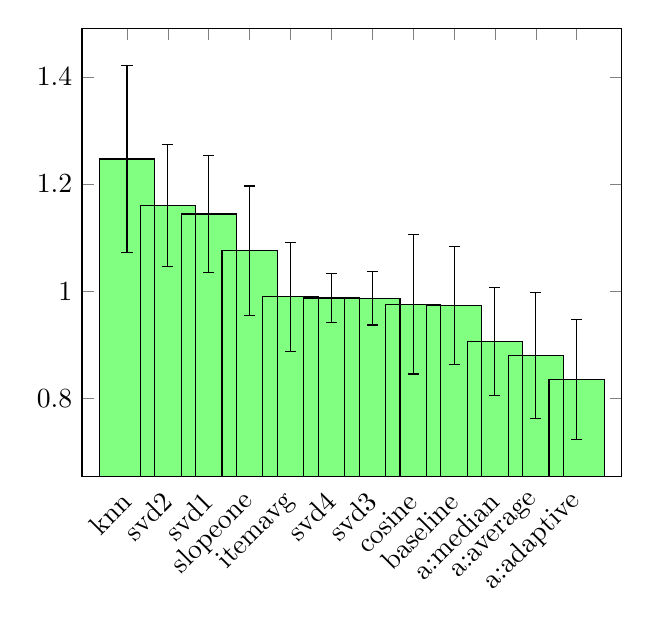
\begin{tikzpicture}

\begin{axis}[
      symbolic x coords={
        knn,svd2,svd1,slopeone,itemavg,svd4,svd3,cosine,baseline,a:median,a:average,a:adaptive},
      xtick=data,
      x tick label style={rotate=45,anchor=east,yshift=-0.5em,xshift=-0.2em},
      bar width=20pt
    ]

    \addplot [ybar,fill=green!50,error bars/.cd,y dir=both,y explicit] coordinates {
      (knn, 1.2467) +- (0,0.17435) 
      (svd2, 1.1605) +- (0,0.11385)
      (svd1, 1.1441) +- (0,0.10985)
      (slopeone, 1.0756) +- (0,0.12075)
      (itemavg, 0.9895) +- (0,0.10115)
      (svd4, 0.9873) +- (0,0.0462)
      (svd3, 0.9865) +- (0,0.04955)
      (cosine, 0.9754) +- (0,0.12975)
      (baseline, 0.9738) +- (0,0.1098)
    %};
    %\addplot [ybar,fill=blue!50] coordinates {
      (a:median, 0.9065) +- (0,0.10025)
      (a:average, 0.8801) +- (0,0.1172)
      (a:adaptive, 0.8352) +- (0,0.11125)
    };
\end{axis}

\end{tikzpicture}
\caption[Average RMSE Plot]{
  Average RMSE plot: This plot shows the average RMSE for each method, and each aggregation method (denoted "a:").
  The actual numbers are given in Table \ref{table:results:e1}.
  The error bars indicate the standard deviation of each method.
  Note the scale on the y-axis --- the errors are not as pronounced as they might seem. 
  See also Figure \ref{plot:datasets}.
}
\label{plot:rmse}
\end{figure}




%\begin{figure}[p]
  \centering
  \subfloat[Experiment 1]{\label{fig:rmse:e1}
\pgfplotsset{width=\textwidth,height=8cm}
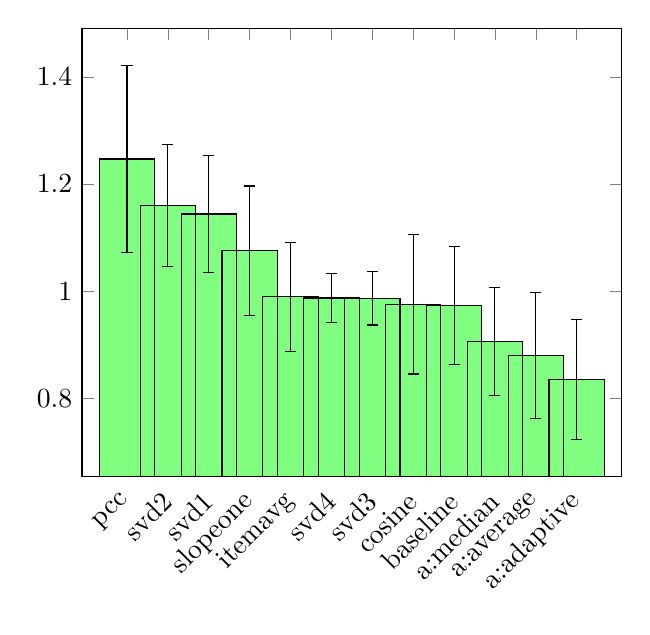
\begin{tikzpicture}
\begin{axis}[
      symbolic x coords={
        pcc,svd2,svd1,slopeone,itemavg,svd4,svd3,cosine,baseline,a:median,a:average,a:adaptive},
      xtick=data,
      x tick label style={rotate=45,anchor=east,yshift=-0.5em,xshift=-0.2em},
      bar width=20pt
    ]
    \addplot [ybar,fill=green!50,error bars/.cd,y dir=both,y explicit] coordinates {
      (pcc, 1.2467) +- (0,0.17435) 
      (svd2, 1.1605) +- (0,0.11385)
      (svd1, 1.1441) +- (0,0.10985)
      (slopeone, 1.0756) +- (0,0.12075)
      (itemavg, 0.9895) +- (0,0.10115)
      (svd4, 0.9873) +- (0,0.0462)
      (svd3, 0.9865) +- (0,0.04955)
      (cosine, 0.9754) +- (0,0.12975)
      (baseline, 0.9738) +- (0,0.1098)
    %};
    %\addplot [ybar,fill=blue!50] coordinates {
      (a:median, 0.9065) +- (0,0.10025)
      (a:average, 0.8801) +- (0,0.1172)
      (a:adaptive, 0.8352) +- (0,0.11125)
    };
\end{axis}
\end{tikzpicture}}

\vspace{1em}
 
  \subfloat[Experiment 2]{\label{fig:rmse:e2}
\pgfplotsset{width=\textwidth,height=8cm}
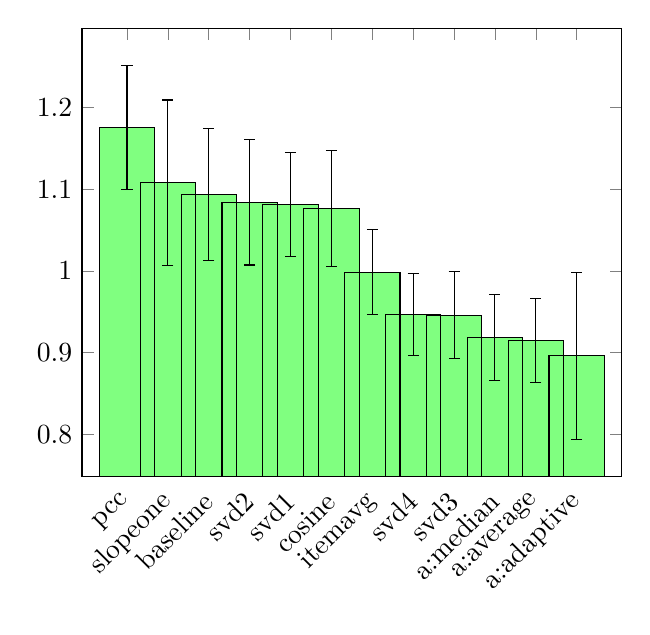
\begin{tikzpicture}
\begin{axis}[
      symbolic x coords={
        pcc,slopeone,baseline,svd2,svd1,cosine,itemavg,svd4,svd3,a:median,a:average,a:adaptive},
      xtick=data,
      x tick label style={rotate=45,anchor=east,yshift=-0.5em,xshift=-0.2em},
      bar width=20pt
    ]
    \addplot [ybar,fill=green!50,error bars/.cd,y dir=both,y explicit] coordinates {
      (pcc, 1.175422) +- (0,0.0758) 
      (slopeone, 1.10813) +- (0,0.101039)
      (baseline, 1.09358) +- (0,0.080985)
      (svd2, 1.084098) +- (0,0.076837)
      (svd1, 1.08128) +- (0,0.063377)
      (cosine, 1.076532) +- (0,0.0709)
      (itemavg, 0.99843) +- (0,0.052021)
      (svd4, 0.947158) +- (0,0.050071)
      (svd3, 0.946024) +- (0,0.052801)
    %};
    %\addplot [ybar,fill=blue!50] coordinates {
      (a:median, 0.918404) +- (0,0.052478)
      (a:average, 0.915036) +- (0,0.051037)
      (a:adaptive, 0.896294) +- (0,0.102056)
    };
\end{axis}
\end{tikzpicture}}

\vspace{1em}

  \caption[Plots of Results for Experiments 1 \emph{\&} 2]{
    Plots of the average RMSEs for Experiments 1 \emph{\&} 2.
    The actual numbers are given in Tables \ref{table:results:e1}
    \emph{\&} \ref{table:results:e2}.
    Note the scale on the y-axis --- the errors are not as pronounced as they might seem. 
  }
  \label{plot:rmse}
\end{figure}




\begin{figure}
\center

\pgfplotsset{width=\textwidth,height=8cm}
\pgfplotsset{every axis/.append style={
thick,
tick style={semithick}}}

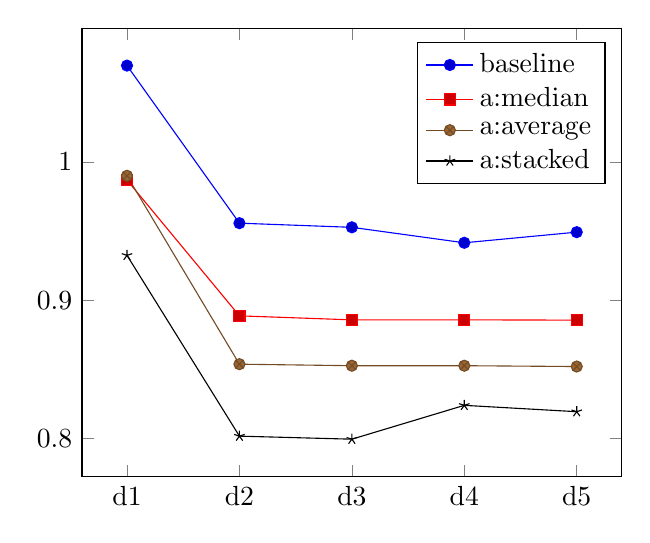
\begin{tikzpicture}

\begin{axis}[
  stack plots=false,
  enlarge x limits=true,
  symbolic x coords={d1,d2,d3,d4,d5},
  xtick=data,
  legend style={
    cells={anchor=west},
    legend pos=north east,
  }
]

\addplot coordinates {
(d1, 1.0698)
(d2, 0.9557)
(d3, 0.9527)
(d4, 0.9415)
(d5, 0.9492)
};
\addlegendentry{baseline}


\addplot coordinates {
(d1, 0.9869)
(d2, 0.8886)
(d3, 0.8857)
(d4, 0.8857)
(d5, 0.8855)
};
\addlegendentry{a:median}
 
\addplot coordinates {
(d1, 0.9900)
(d2, 0.8536)
(d3, 0.8525)
(d4, 0.8525)
(d5, 0.8519)
};
\addlegendentry{a:average}
 
\addplot coordinates {
(d1, 0.9324)
(d2, 0.8015)
(d3, 0.7993)
(d4, 0.8238)
(d5, 0.8192)
};
\addlegendentry{a:stacked}

\end{axis}
\end{tikzpicture}

\caption[RMSE Variations]{
  RMSE Variations: This plot shows that, while the standard deviation of each method may be high,
  this has more to do with the selected dataset than with their performance in comparison with each other.
  The performance of each of the aggregate methods, as well as the baseline standard method,
  follow similar performance paths across the disjoint datasets.
}
\label{plot:datasets}
\end{figure}






Let us take a look at the standard deviation measures from the different methods.
As seen in Figure \ref{plot:rmse}, 
most of the methods, including the stacked models,
exhibit quite a lot of variation in their results.
If these variations occured as a result of unstable
predictions of the same dataset, this would be a substantial problem,
resulting in unreliable predictions.
However, as seen in Figure \ref{plot:datasets},
the standard deviation is mostly caused by the differing
performance across the varying datasets.
As we see, the performance of each of the aggregation methods,
as well as the best performing standard recommender,
follow each other closely. At the same time,
performance varies across the different datasets,
which results in high values for $\sigma$.

What does this mean for hypotheses H1 and H2?
Expressed in terms of this experiment,
H1 posits that stacked recommenders should outperform each of the standard modeling methods
in Table \ref{table:results:e1}.
The adaptive methods blend the results of multiple predictors by estimating the accuracy
on a per-item and per-user basis, satisfying the formulation of H1.

By outperform we mean that our model should have a lower
mean RMSE score than the other singular methods. As we can see in Table \ref{table:results:e1:sum},
\emph{H1 is confirmed for these methods and this dataset}.
While we can not generalize too much on this basis, 
the fact that this dataset is a common testing ground for recommender systems,
that RMSE is the de facto measure for determining performance,
and because of our 5-fold cross-validation, the results allow us 
to confirm hypothesis H1 in these conditions, and likely for other, similar scenarios.
We shall discuss this in Chapter \ref{chap:discussion}.

Similarly, expressed in the same terms, H2 posits that 
our stacked recommenders should outperform the aggregation approaches
given in Table \ref{table:results:e1}.
The \emph{median} and \emph{average} aggregation methods
serve as globalized and generalized aggragation methods,
Stacked recommenders are adaptive in that each prediction is 
aggregated based on the current user and item,
satisfying the language of H2.

As we can see in Table \ref{table:results:e1:sum},
\emph{H2 is confirmed for these methods and this dataset}.
However, as our collection of aggregation methods is a lot simpler
than our collection of recommender systems, the strength of this combination
is notably weaker than that of H1.
Still, the fact that a stacked recommender outperforms these simple aggregation
approaches is a positive result warranting further experiments.
This will also be discussed in Chapter \ref{chap:discussion}.

It would seem then that, based on our experiments, available data
and assumptions of evaluation measures, both H1 and H2 are confirmed.
Our adaptive aggregation approach outperforms both standard recommender
methods and simple generalized aggregation methods.
Notably, our approach is more complex than the methods it outperforms,
so the question whether the methods performance is worth its extra complexity becomes important.
We shall discuss this, and other implications of these results in the next chapter.
For now, let us proceed to the second experiment and hypothesis H3.

\clearpage

\section{Rank Aggregation}

\begin{table}[h]
  \centering 

  \begin{tabular*}{0.9\textwidth}{ r l p{8cm} }
    \multicolumn{3}{l}{Results and their IR ranking score for the query [\emph{``new york'' or washington}]:}\\
    \toprule
    \emph{\#} & \emph{score} & \emph{title}\\
    \midrule
    1 & 2.8419  &  New York Cop (1996)                    \\
    2 & 2.8419  &  King of New York (1990)                \\
    3 & 2.8419  &  Autumn in New York (2000)              \\
    4 & 2.8419  &  Couch in New York                      \\
    5 & 2.4866  &  Escape from New York (1981)            \\
    6 & 2.4866  &  All the Vermeers in New York (1990)    \\
    7 & 2.1314  &  Home Alone 2: Lost in New York (1992)  \\
    8 & 1.0076  &  Saint of Fort Washington               \\
    9 & 1.0076  &  Washington Square (1997)               \\
    10& 0.8816  &  Mr. Smith Goes to Washington (1939)    \\
    \bottomrule
  \end{tabular*}

  \vspace{1em} 

  \begin{tabular*}{0.9\textwidth}{ r l p{8.5cm} l }
    \multicolumn{4}{l}{Predicted ratings from the adaptive recommenders method for each item:}\\
    \toprule
    \emph{\#} & \emph{score} & \emph{title} & $\Delta_{IR}$\\
    \midrule
    1 & 3.7255  &  Mr. Smith Goes to Washington (1939)    & \color{green} $\uparrow$ 9 \\
    2 & 3.1430  &  Escape from New York (1981)            & \color{green} $\uparrow$ 3 \\
    3 & 3.0003  &  King of New York (1990)                & \color{red} $\downarrow$ 1 \\
    4 & 2.9498  &  Washington Square (1997)               & \color{green} $\uparrow$ 5 \\
    5 & 2.7258  &  Saint of Fort Washington               & \color{green} $\uparrow$ 3 \\
    6 & 2.6862  &  Couch in New York                      & \color{red} $\downarrow$ 2 \\
    7 & 2.6380  &  All the Vermeers in New York (1990)    & \color{red} $\downarrow$ 1 \\
    8 & 2.1601  &  Home Alone 2: Lost in New York (1992)  & \color{red} $\downarrow$ 1 \\
    9 & 1.7241  &  Autumn in New York (2000)              & \color{red} $\downarrow$ 6 \\
    10& 0.0     &  New York Cop (1996)                    & \color{red} $\downarrow$ 6 \\
    \bottomrule
  \end{tabular*}

  \vspace{1em} 

  \begin{tabular*}{0.9\textwidth}{ r l p{8.5cm} l }
    \multicolumn{4}{l}{Final results list with IR and adaptive predictions combined:}\\
    \toprule
    \emph{\#} & \emph{score} & \emph{title} & $\Delta_{IR}$ \\
    \midrule
    1 & 5.8422  &  King of New York (1990)                & \color{green} $\uparrow$ 1 \\
    2 & 5.6297  &  Escape from New York (1981)            & \color{green} $\uparrow$ 3 \\
    3 & 5.5281  &  Couch in New York                      & \color{green} $\uparrow$ 1 \\
    4 & 5.1247  &  All the Vermeers in New York (1990)    & \color{green} $\uparrow$ 2 \\
    5 & 4.6072  &  Mr. Smith Goes to Washington (1939)    & \color{green} $\uparrow$ 5 \\
    6 & 4.5661  &  Autumn in New York (2000)              & \color{red} $\downarrow$ 3 \\
    7 & 4.2915  &  Home Alone 2: Lost in New York (1992)  & \color{black} $=$ \\
    8 & 3.9575  &  Washington Square (1997)               & \color{green} $\uparrow$ 1 \\
    9 & 3.7334  &  Saint of Fort Washington               & \color{red} $\downarrow$ 1 \\
    10& 2.8419  &  New York Cop (1996)                    & \color{red} $\downarrow$ 9 \\
    \bottomrule
  \end{tabular*}

  \vspace{1em}
  \caption[Complex IR Query]{
    Complex IR query:
    The first table shows the results returned by our IR model, defining the item-space for the following tables.
    The middle table shows the predicted ratings for each of the items in the results set.
    $\Delta_{IR}$ shows how much each item has moved compared to the initial IR results.
    Notably, the recommenders were not able to predict the rating for the movie "new york cop",
    which results in a low final placement for this item.
  }
  \label{table:rank:washington}
\end{table}


\afterpage{\clearpage}

While the previous experiment was a quantitative exploration of RMSE values,
this experiment will focus on qualitative traits of rank aggregation.
In particular we wish to see how our method can perform personalized search.

The MovieLens dataset fit the needs of this experiment.
Searching through movies is a scenario where the actual predicted
rating of each movie would be a welcome signal for ranking the results.
In other words, we have a database of movies the user wishes to search through,
where the results are ranked both by how well they match the free text query,
and according to the predicted rating of each movie for the current user.

Hypothesis H3 states that 
{
  \itshape
  the result set from an information retrieval query
  can be adaptively personalized by layering recommenders.
}
We wish to check if the prediction algorithm
in Listing \ref{code:rank:prediction} performs personalized search
in a meaningful way.
There are a few important limitations to this experiment:

\begin{itemize}
  \item 
    We are not interested in measuring the actual performance of the IR system.
    It us assumed that the IR model returns items relevant to the current query,
    ranked by their individual relevance.
  \item
    We are not interested in measuring the performance of the resulting personalized search.
    This experiment will only show whether or not personalized search is achievable
    by using adaptive recommenders, as per our hypothesis.
\end{itemize}

\begin{comment}
\begin{table}[b]
  \centering
  \begin{tabular*}{0.7\textwidth}{ l l l l }
    \toprule
      ~ & 
      \emph{query} &
      \emph{scores} &
      \emph{IR weight} \\
    \midrule
    
    1 &
    ["new york or washington"] &
    combined &
    $1.0$ \\

    2 &
    [star trek] &
    combined &
    $0.3$ \\

    3 &
    [paris] &
    ratings &
    $0.0$ \\

    4 &
    [1998] &
    ratings &
    $0.0$ \\

    \bottomrule 
  \end{tabular*}
  \caption[List of Ranking Experiments]{List of ranking tests in this section.}
  \label{table:experiments:rank}
\end{table}
\end{comment}

There are many ways of determining the accuracy of a personalized search
algorithm, such as the mean average precision of the results list
(the mean of the precision average over a set of queries).
However, these are subjective measures based on relevance judgements from each user.
Our hypothesis only states that our algorithm should be usable for such 
a system, which is what we shall explore in this section.
To quantitatively measure the performance of personalized search,
one would need detailed query logs, user profiles and click-through information,
which we have no access to.

Of course, any recommender system can be used for personalized search.
The interesting bit in regards to adaptive recommenders is what 
happens under the hood. First, the information retrieval score 
is itself treated as an input signal, just as the user modeling methods.
Second, by using adaptive recommenders, the user is in control of which
methods that actually determine how the final results are ranked.
We shall take a look at four use cases with to see how our algorithm
performs in a number of scenarios. Each case presents 
a query and shows how a certain IR weight influences the final ranking.

The IR weight is the ratio multiplied with the IR score 
before the adaptive recommender scores are incorporated
(see Listing \ref{code:rank:prediction}).
The actual choice of weight depends on scale of scores
returned by the IR method.
If the scores are on the same scales as the ratings themselves,
an IR weight of $1$ signifies that the IR score
should have equal importance as each recommender score.
Any higher, and the IR model should be prioritized above the recommenders.
Any lower, and the recommender scores will dominate the initial IR rankings.

In other words, the actual IR weight must
be calculated based on the scale of the IR scores.
In this chapter, the scores returned by our IR
model is normalized to the scale of our ratings (1-5).

We will consider the following use cases:
(1) searching multiple topics,
(2) searching for a series of movies,
(3) searching for one particular topic, and
(4) searching for a particular attribute.

\begin{table}[h]
  \centering 

  \begin{tabular*}{0.9\textwidth}{ r l p{8cm} }
    \multicolumn{3}{l}{Results and their IR ranking score for the query \emph{star trek}:}\\
    \toprule
    \emph{\#} & \emph{score} & \emph{title}\\
    \midrule
    1 & 4.2288 & Star Trek: Generations                 \\
    2 & 3.7002 & Star Trek: First Contact               \\
    3 & 3.7002 & Star Trek: The Wrath of Khan           \\
    4 & 3.7002 & Star Trek: The Motion Picture          \\
    5 & 3.1716 & Star Trek VI: The Undiscovered Country \\
    6 & 3.1716 & Star Trek III: The Search for Spock    \\
    7 & 3.1716 & Star Trek IV: The Voyage Home          \\
    8 & 3.1716 & Star Trek V: The Final Frontier        \\
    9 & 0.9670 & Star Wars                              \\
    10& 0.9670 & Lone Star                              \\
    \bottomrule
  \end{tabular*}

  \vspace{1em} 

  \begin{tabular*}{0.9\textwidth}{ r l p{8.5cm} l }
    \multicolumn{4}{l}{Predicted ratings from the stacked recommender method for each item:}\\
    \toprule
    \emph{\#} & \emph{score} & \emph{title} & $\Delta_{IR}$\\
    \midrule
    1 & 4.8232 & Star Wars                              & \color{green} $\uparrow$ 9 \\
    2 & 4.6016 & Lone Star                              & \color{green} $\uparrow$ 8 \\
    3 & 4.2192 & Star Trek: The Wrath of Khan           & \color{black} $=$ \\
    4 & 4.0324 & Star Trek: First Contact               & \color{red} $\downarrow$ 2 \\
    5 & 3.8667 & Star Trek: Generations                 & \color{red} $\downarrow$ 4 \\
    6 & 3.7100 & Star Trek IV: The Voyage Home          & \color{green} $\uparrow$ 1 \\
    7 & 3.5604 & Star Trek VI: The Undiscovered Country & \color{red} $\downarrow$ 2 \\
    8 & 3.4420 & Star Trek: The Motion Picture          & \color{red} $\downarrow$ 4 \\
    9 & 3.4242 & Star Trek III: The Search for Spock    & \color{red} $\downarrow$ 3 \\
    10& 2.5249 & Star Trek V: The Final Frontier        & \color{red} $\downarrow$ 2 \\
    \bottomrule
  \end{tabular*}

  \vspace{1em} 

  \begin{tabular*}{0.9\textwidth}{ r l p{8.5cm} l }
    \multicolumn{4}{l}{Final results list with IR and stacked predictions combined:}\\
    \toprule
    \emph{\#} & \emph{score} & \emph{title} & $\Delta_{IR}$ \\
    \midrule
    1 & 5.5507  &    Star Trek: The Wrath of Khan            & \color{green} $\uparrow$ 2 \\
    2 & 5.5205  &    Star Trek: First Contact                & \color{black} $=$ \\
    3 & 5.3157  &    Star Trek: Generations                  & \color{red} $\downarrow$ 2 \\
    4 & 5.1187  &    Star Wars                               & \color{green} $\uparrow$ 5 \\
    5 & 4.9744  &    Star Trek IV: The Voyage Home           & \color{green} $\uparrow$ 2 \\
    6 & 4.7596  &    Star Trek III: The Search for Spock     & \color{black} $=$ \\
    7 & 4.7595  &    Star Trek: The Motion Picture           & \color{red} $\downarrow$ 3 \\
    8 & 4.7553  &    Star Trek VI: The Undiscovered Country  & \color{red} $\downarrow$ 3 \\
    9 & 4.6376  &    Lone Star                               & \color{green} $\uparrow$ 1 \\
    10& 4.0934  &    Star Trek V: The Final Frontier         & \color{red} $\downarrow$ 2 \\
    \bottomrule
  \end{tabular*}
  \vspace{1em}
  \caption[Adaptive Rank Rescoring]{
    These three table show adaptive rank rescoring for the query "star trek".
    In this example, an IR weight of $0.3$ was used, instructing the algorithm to
    put about the same confidence in the IR score and recommender scores.
    In other words, each score is considered an input signal, and each 
    signal is weighted the same.
  }
  \label{table:rank:startrek}
\end{table}


\afterpage{\clearpage}

(1) Let us start with a simple use case:
a user wishes to find movies about two separate topics, ranked by 
query match and predicted ratings.
This is a realistic use case, for example if a user is interested
in a few topics and wants to see the movie within these categories
he or she will probably like the most.
The IR algorithm takes care of finding the items within the categories,
while the adaptive recommenders finds the most enjoyable movies,
according to the metrics most preferred by this user in the past.

Table \ref{table:rank:washington} shows this use case and how our algorithm performs.
The results are for the query [\emph{"new york" or washington}].
The first table shows the IR scores for the first 10 results,
and their rank (position in the list) according to these scores.
The second table shows the predicted rankings for each of these items.
Finally, the third table shows the ranking after the IR scores
and predicted ratings have been combined.
The final column shows how each item have moved in relation to the 
IR results list.

In this run of the algorithm, the IR weight ($w_{IR}$) was set to $1.0$,
instructing the algorithm place about the same importance on the IR score
and the predicted ratings. As we can see in the last section of 
Table \ref{table:rank:washington} the final result list is a blend
of the IR rankings and prediction rankings.
In other words, we have achieved personalized search: the results
from the IR method are re-ranked according to personal preferences.


(2) Let us consider another use case:
A user wishes to see a movie in a certain series of movies,
but does not know which one. In this case, the IR method can find all movies within this series,
while the recommender systems ranks the result list according to the user's preferences.

Table \ref{table:rank:startrek} shows the intermediary and final ranking
for the query [\emph{star trek}], which refers to a movie series.
The IR method returns all items that match this query,
and the recommenders predict the rating for each of these items.
However, since the IR method only ranks results based on how well they match the query,
and the recommenders only care about the predicted rating, the combined result
list can get the best of both worlds:
the top ranked items are the ones that both match the query \emph{and}
are probable good fits for the current user.

(3) What happens when the IR weight is set to $0$?
In this use case, the predicted ratings alone sort the final list.
Consider the following use case:
A user wishes to see a movie related to a certain topic, e.g. a city.
Table \ref{table:rank:paris} shows two results lists for the query [\emph{paris}].
On the left are the standard ranking as returned by the IR model for this query,
along with their respective scores.
On the right we see the same results, re-ranked by user preferences.

For simple one-word queries, ignoring the IR score seems to give us the desired effect.
When we can be sure that each item returned by a search have the same textual relevance
(IR score), the IR method does not have any more information on which to rank
the results. The ranking then becomes the task of the recommender systems.
By employing adaptive recommenders, the results are not only ranked by 
one or more recommenders as chosen by the system, but by those of the recommenders
best suited to the current user. At the same time, each of these recommenders
are used differently for each item in the list, based on how well they have
performed for each item in the past.

(4) As we can see, ignoring the IR score gives us quite a different algorithm.
Now, the search part is only performed to constrain the item-space worked
on by the recommender systems.
Another example of this is shown in Table \ref{table:rank:year}.
In this scenario, the user wishes to see a movie from a certain year,
and issues the query [\emph{1998}].
Naturally, the IR algorithm returns a whole lot of items, and each can
be said to be perfect answers to the algorithm -- each movie
was made in 1998.

In this case, setting the IR weight to $0$ allows us to rank the results
purely by predicted preference, which makes sense when the IR algorithm
can not rank the results in any meaningful way.
Note that the items in the left and right table are non-overlapping.
This is because only the first 10 results are shown.
The IR model returns a large number of items,
all with the same ranking score.
The recommender systems do the final ranking, and actually
push every item in the top 10 IR ranking 
below the top 10 final results.

\begin{table}[t]
  \centering 
  \begin{minipage}{0.49\textwidth}
    \centering 

  \begin{tabular*}{\textwidth}{ r l l }
    \toprule
    \emph{\#} & \emph{score} & \emph{title}\\
    \midrule
    1 & 3.0149  &  An American in Paris       \\
    2 & 3.0149  &  Paris Is Burning           \\
    3 & 3.0149  &  Paris - Texas              \\
    4 & 3.0149  &  Paris Was a Woman          \\
    5 & 3.0149  &  Forget Paris               \\
    6 & 3.0149  &  Window to Paris            \\
    7 & 3.0149  &  Jefferson in Paris         \\
    8 & 3.0149  &  Paris - France             \\
    9 & 2.6648  &  Rendezvous in Paris        \\
    10& 2.2611  &  Last Time I Saw Paris  \\
    \bottomrule
  \end{tabular*}
\end{minipage} 
\hfill 
\begin{minipage}{0.49\textwidth}
  \begin{tabular*}{\textwidth}{ r l l l }
    \toprule
    \emph{\#} & \emph{rating} & \emph{title} & $\Delta$\\
    \midrule
    1 & 3.5277 &  An American in Paris        & \color{black} $=$ \\
    2 & 3.3416 &  Forget Paris                & \color{green} $\uparrow$ 3 \\
    3 & 3.2037 &  Paris - Texas               & \color{black} $=$ \\
    4 & 3.1870 &  Window to Paris             & \color{green} $\uparrow$ 2 \\
    5 & 3.1409 &  Paris Is Burning            & \color{red} $\downarrow$ 3 \\
    6 & 3.1059 &  Last Time I Saw Paris       & \color{green} $\uparrow$ 4 \\
    7 & 2.7940 &  Rendezvous in Paris         & \color{green} $\uparrow$ 2 \\
    8 & 2.2964 &  Paris - France              & \color{black} $=$ \\
    9 & 1.7984 &  Jefferson in Paris          & \color{red} $\downarrow$ 2 \\
    10& 0.9420 &  Paris Was a Woman           & \color{red} $\downarrow$ 6 \\
    \bottomrule
  \end{tabular*}
  \end{minipage} 
  \vspace{1em}
  \caption[Completely Adaptive Ranking]{
    Completely adaptive ranking: With the IR weight set to $0$,
    the adaptive recommender is alone responsible for sorting the results.
    In this example, the IR model returns a list of items for the query "paris",
    and the adaptive user models sorts the results according to the user's preferences.
    The top 10 results are shown.
  }
  \label{table:rank:paris}
\end{table}



As we have seen in this section, adaptive recommenders can provide personalized search
in multiple ways. 
Because of this, hypotheses H3 is confirmed for these use cases with our dataset.
By varying the IR weight we can create quite a range of systems:
On the one hand, an IR weight of 0 will let the recommenders do all the ranking.
On the other hand, by increasing the IR weight, the recommenders will carefully
adapt parts of the IR results list by moving some of the items.

\begin{table}[t]
  \centering 
  \begin{minipage}{0.49\textwidth}
    \centering 

  \begin{tabular*}{\textwidth}{ r l l }
    \toprule
    \emph{\#} & \emph{score} & \emph{title}\\
    \midrule
    1 &  2.7742  &  Fallen (1998)      \\
    2 &  2.7742  &  Sphere (1998)      \\
    3 &  2.7742  &  Phantoms (1998)    \\
    4 &  2.7742  &  Vermin (1998)      \\
    5 &  2.7742  &  Twilight (1998)    \\
    6 &  2.7742  &  Firestorm (1998)   \\
    7 &  2.7742  &  Palmetto (1998)    \\
    8 &  2.7742  &  The Mighty (1998)  \\
    9 &  2.7742  &  Senseless (1998)   \\
    10&  2.7742  &  Everest (1998)     \\
    \bottomrule
  \end{tabular*}
\end{minipage} 
\hfill 
\begin{minipage}{0.49\textwidth}
  \begin{tabular*}{\textwidth}{ r l l l }
    \toprule
    \emph{\#} & \emph{rating} & \emph{title}\\
    \midrule
    1 &  3.8694  &  Apt Pupil (1998)            \\
    2 &  3.4805  &  The Wedding Singer (1998)   \\
    3 &  3.1314  &  Fallen (1998)               \\
    4 &  3.1225  &  Tainted (1998)              \\
    5 &  2.9442  &  Blues Brothers 2000 (1998)  \\
    6 &  2.9046  &  Sphere (1998)               \\
    7 &  2.8842  &  Desperate Measures (1998)   \\
    8 &  2.8798  &  Firestorm (1998)            \\
    9 &  2.8633  &  Vermin (1998)               \\
    10&  2.8511  &  The Prophecy II (1998)      \\
    \bottomrule
  \end{tabular*}
  \end{minipage} 
  \vspace{1em}
  \caption[Ranking Many Results]{
    Ranking many results: 
    In this example, the user search for the query "1998", to get movies from that year.
    The top 10 of these are shown in the left table. As this query matches a lot of 
    movies, the IR method returns a large number of results. By setting the IR weight to $0$,
    and letting the stacked user models do the ranking, the top 10 results change completely,
    while still being good matches for the current query.
  }
  \label{table:rank:year}
\end{table}


We have not considered which IR weight or other parameters would result in the best performing
personalized search system.
However, this is completely dependent on the type of system and types of queries.
By varying the IR weight, a number of different systems that work for different use cases
can be constructed. For systems with simple one-word queries, setting the weight
to $0$ leaves ranking to the recommenders.
For systems with more complex queries, an IR weight of $1.0$ 
orders items both by IR score and predicted rating.
Naturally, this weight is a defining characteristic of any 
personalized search based on adaptive recommenders.

The performance of personalized search is hard to judge without
extensive query logs with click-through information.
While we had no access to such data, 
we have been able to show that adaptive recommenders
work well for personalized search.
This positive result for Experiment 3 confirms hypothesis H3,
at least for this dataset, this IR system and our chosen recommender algorithms.

The next chapter will discuss the implications and limitation of our results.



%\hr
%
%\noindent
%In this chapter, we have seen what stacked recommenders are capable of.
%We confirmed hypotheses H1 and H2 by showing that this technique
%can outperform both standard recommender systems and 
%simple aggregation methods. As seen in the previous section,
%H3 was confirmed by showing how stacked recommenders can provide
%personalized search together with an IR model.
%The next chapter will discuss these findings and their respective implications.



    \chapter{Discussion \emph{\&} Conclusion}
      \label{chap:discussion}

This chapter will discuss the implications and limitations of our results.
While our hypotheses may be confirmed,
it is important to clarify what we have actually found out,
and what limits there is to this knowledge.
We will also summarise the contributions of this thesis,
and suggest possible future work.


\section{Implications}      

Our central assumption is that modern recommender systems 
are constrained by their misplaced subjectivity.
Each system selects some measures to model its users, 
based on how they think each user and item \emph{should} be modeled.
We believe this selection should be left to each user:
different users and items will require adaptive recommender algorithms that
consider the context before making predictions.

Adaptive recommenders can help solve this problem.
In a collection of possible recommender algorithms, each is adaptively used based 
on how well it performs for the item and user in question.
The experiments of the previous chapter shows the promise of this technique.
However, there are lots of use cases not yet considered.

It should be clear that adaptive recommenders would work best in situations where
we have a wide range of diverse algorithms that can infer the relevance of an item to a user.
For users, social connections is a good example. Whether or not social connections should influence
recommendations or personalized search results is a contentious topic.
Naturally, a system where each user's personal opinion determines if these connections are used is desireable.

This implication extends to the items that should be recommended:
As evident by the field of information retrieval,
there exists many ways of considering the relevance of an item. 
Each of these algorithms can be based on a number of attributes, for example
temporal information, geography, sentiment analysis, topic or keywords.
It is not a huge leap to assume that each of these algorithms may have
varying levels of accuracy for each individual item.
Adaptive recommenders can help solve this problem by adaptively 
combining the recommenders based on individual item performance.

Hypothesis H1 was confirmed by showing that adaptive recommenders
can outperform standard single-approach recommenders.
We achieved lower total RMSE scores across each of our datasets,
which would imply that adaptive recommenders
reliably performs better than our tested standard recommenders.
However, the real test would be to use our approach
in a situation with even more differing recommender systems.


Hypothesis H2 was confirmed by showing that adaptive recommenders
can outperform simple, generalized aggregation approaches.
While our aggregators were simple,
this result is promising.
However, it remains to test our method
against more complex generalized aggregation functions.

Hypothesis H3 was confirmed by showing that our approach
can be used to provide personalized search.
While we did not strictly evaluate the quantitative performance
of this approach, our results show that different
prioritisations of the IR scores can cope with many different use cases.
The key insight is that the IR score can be seen as a signal
on the same level as the adaptive recommenders,
gaining the power of query matching and relevance matching
in the same results set.

With adaptive recommenders, both the methods layer and the adaptive layer consists of standard recommender algorithms.
Because we use ratings matrices for the taste models and error matrices for the weight estimations,
we can use the same algorithms for both tasks.
Using known algorithms for this new task is beneficial:
they are known to work, enjoy multiple implementations
and are already understood and battle-tested in many different systems.


\section{Limitations}

There are some important general limitations to our research
related to the 
(1) complexity of our method, 
(2) our choice of data and evaluation metrics, 
(3) the general usefulness of this approach, and
(4) common issues with recommender systems.

(1) Complexity: As our approach is more complicated than standard recommenders,
it is worth questioning if its gains are worth the extra complexity.
This depends on the basic recommenders that are to be combined.
If the system is made up by many different recommenders,
that each user might place varying importance on,
and that may have varying success with each item,
adaptive recommenders may provide gains in accuracy.

On the other hand, if the recommenders are simple in nature,
and look at similar patterns in the data,
generalized aggregation methods might be more applicable.
Clearly, the performance gains in our experiments
are not substantial enough to declare anything without reservation.
While we believe this technique has potential,
without real-world success stories, it is hard
to suggest that our method is particularly better
than a simple standard recommender.

(2) Evaluation: we chose traditional datasets and evaluation metrics
to validate the adaptive recommenders technique.
While our initial results are promising, it is important to stress
that this is only one test on one dataset. Considering the vast scope
of applicable data, and the number of ways these results many be 
evaluated, the results must be seen for what they are:
initial and preliminary explorations of a new technique
that has yet to be proved useful in the real world.

As mentioned in Chapter \ref{chap:theory}, the scale of known ratings is another concern.
When we have a set of explicit ratings given by users, these are often
given in discrete steps, and not on a continuous scale.
As known from the field of statistics, when using ordinal scales,
the significance of each steps are not necessarily equal.
For instance, on a scale from 1 through 5, the difference
between 2 and 3 might not be as significant as the difference between 4 and 5.
This is a limitation of many recommender system, apparent by the algorithms they use:
most do not consider the implications of ordinal data.
Naturally, in a real-world system, this limitation has to be considered.

(3) Usefulness:
When considering the additional complexity of our approach,
a natural response is whether or not current approaches
to recommender systems are good enough.
We do not think so. Information overload is such a nuanced problem 
that the only solution lines in intelligent, adaptive systems.
However, as most of today's recommender systems 
perform quite simple tasks, they may be more
than good enough for their purpose.

This will always be a trade-off, between complexity and required accuracy.
As in many other cases, each of the systems described in this thesis
have their use cases. In the end, the requirements of each system
must decide which method best suit their needs.

(4) Common issues:
The topic of recommenders and adaptive systems in general
raise a number of questions which is outside the scope of this thesis.
For example, user privacy is a big issue.
Whenever we have a system that tries to learn the tastes, habits and
traits of its users, how each user will react to this must be considered.
This is often a trade-off between adaptability and transparency.
The most adaptive systems will not always be able to explain to the users
what is going on and what it knows about each person,
especially when dealing with emergent behavior based on 
numerical user models.

Another important issue is the usability of autonomous interfaces.
Whenever recommenders are used for more than simple lists of items,
there is a question of how easy the resulting system will be to use.
As mentioned in Chapter \ref{chap:theory},
unpredictability is the enemy of usability.
Creating an autonomous system that is also
predictable is a serious challenge, and a common trade-off.

While a thorough discussion of privacy and usability is 
outside our scope, they are both important limitations to considered
when using a recommender system.

In addition to these general limitations, 
each experiment has its own limiting factors.

Hypothesis H1 was only tested against a limited number of standard recommenders.
The key word is standard. These recommenders were not heavily customized
to fit the available data. As in much of machine learning,
achieving relatively good performance is quite simple.
Any improvements above this standard requires deep domain knowledge,
and methods customized to the problem at hand.
In an actual system, the adaptive recommenders should be tested
against carefully selected standard recommenders,
optimized for the current domain.

Hypothesis H2 was only tested against simple aggregators.
Many more complex aggregations are possible.
While our tests show the basic viability of our approach,
more testing against complex aggregation functions
is still required.

Both H1 and H2 was only tested with two datasets, and with a single error measure.
While its true that these datasets and this error measure are the canonical ways
of estimating the performance of recommender systems,
more research is required to further verify these results.
In particular, both datasets exhibit quite homogenous types of items,
while our approach may have different characteristics in scenarios
with widely differing items and users.

Experiment 1 gave better performance results than Experiment 2.
The differing variable was the dataset used in each experiment.
The main difference between the datasets was that in experiment 1,
we had many more items than in Experiment 2.
However, given that the datasets contain different kinds of items,
we can not generalize on this basis alone.
Clearly, our method will perform differently depending on the data in question,
as one would expect.

Hypothesis H3 was only tested in a qualitative way.
Ideally, if one has access to detailed query logs,
user profiles and click-through information,
a quantitative experiment should be performed.
Such an experiment would have to be done
to compare our approach to other ways of performing
personalized search.
However, we believe these initial results
help demonstrate the probable value of our approach
in this domain.

This is the core limitation of Experiment 3.
Before employing personalized search with adaptive recommenders,
this technique should be evaluated towards the result
of other personalized search algorithms.
This will in large part entail setting the IR weight
of our algorithm, which decides how the resulting
ranking functions should sort search results.


\section{Contributions} 

We have made two main contributions with this thesis:
(1) described the latent subjectivity problem and
(2) developed the technique of adaptive recommenders.

(1) The latent subjectivity problem is one we think hinders
standard recommender systems reaching their full potential.
As far as we know, this problem has not been described
in the context of recommender systems.
The main choice for any such system is how to predict unknown ratings.
To do this, a pattern in the available ratings data must be leveraged.
These patterns are plentiful, and their individual performance
depends on each user and item of the system.
Modern aggregation recommenders utilize many patterns, but on a generalized
level, where each user and item is treated the same.
This underlying subjectivity leads to a mismatch between the notions
of whoever developed the systems, and the users and items of the service.

The latent subjectivity problem extends to any ensemble learning system
(as those described in \cite{Polikar2006}) that blends multiple 
algorithms to leverage patterns.
Whenever we have multiple algorithms that work on a set of items
(and possibly users), there is a question of how accurate each
approach will be for each item.
Averaged or generalized weighted approaches will always
chose the combination that performs best \emph{on average},
with little concern to the uniqueness of items (and users).
In other words, this is a comprehensive problem
that may be discovered amongst many machine learning techniques.

(2) Adaptive recommenders is our attempt to solve the latent subjectivity problem.
As far as we know, this type of adaptive prediction aggregation has not been done before.
Chapter \ref{chap:results} showed that an aggregation that combines predictions based
on estimated accuracy can outperform both standard recommenders and simple aggregation approaches.
Our technique is strengthened by the fact that standard recommender algorithms
are used for the accuracy estimations.
This is the core insight of this thesis. 
\emph{By creating error models for each recommender, we can use this to predict
its accuracy for each user/item combination.
These predictions can then be used to weigh each combined algorithm accordingly.}

As far as the latent subjectivity problem extends to any ensemble learning system,
the adaptive aggregation part of adaptive recommenders can be used to 
create better combinations of many types of predictors.
Whenever we have a set of algorithms producing a set of predicted values
based on items, a set of aggregating recommenders can model the probable
errors of these approaches, based on each individual item.
This leads to adaptive ensembles that should outperform generalized approaches.
Because of this, the technique build in this thesis should be 
applicable in situations other than recommender systems.

While the experiments of Chapter \ref{chap:results} show the general viability of adaptive recommenders,
we believe there are greater opportunities in systems where there  are even more diverging
patterns to be leveraged. The prime examples of this are systems that may or may 
not use social connections between users, and systems which predict the 
relevance of widely varying items.


\section{Future Work}      

We have only shown the basic viability of adaptive recommenders,
and how they can outperform traditional approaches on traditional datasets.
This section outlines a few interesting research topics
which may shed more light on the subject.


\emph{(1) Quantitative Performance of Personalized Search:}
We did not test how well adaptive recommenders would work for personalized search.
Our third experiment was a case study, detailing how this might be done.
With more data or test subjects, it would be possible to measure
actual performance gains (or setbacks) by using adaptive recommenders to
achieve personalized search.

To measure the performance of personalized search one would need detailed query logs with click-through information.
By this we mean logs that show the queries from each user, and which search result each user
selected for each query.
These logs can be mined to create implicit ratings matrices, which can be split into
training- and testing sets.
However, as this is outside our scope, and we lack the neccessary data,
we leave this experiment to future research.


\emph{(2) Choosing Different Adaptive Recommenders:}
We chose to use SVD-based recommenders for the adaptive part of our adaptive approach.
The main reason for this is that we are looking for global traits of the data
when performing accuracy estimations. In other words, we wish to identify
clusters of users and items for which each algorithm may or may not be suited.

However, as the adaptive recommenders can utilize any standard recommender system
to model the errors of another recommender, it would be interesting to perform
a more in-depth study of how different choices for the adaptive layer
influence the final system.
There are many more recommenders that also look at global patterns
that might be well suited for this task.

Another interesting question is whether other machine learning methods can be used for the adaptive layer.
For example, using neural networks to estimate non linear aggregation functions for each user would be an interesting approach.
This was attempted earlier in our research, but abandoned when recommenders were found to produce
better results in a more elegant way.


\emph{(3) Using Adaptive Recommenders in Other Domains:}
We chose to use the MovieLens dataset and the RMSE evaluation measure for testing our approach.
The primary reason was to be able to directly evaluate our results towards those of other research thesis.
As this dataset and this error measure is widely used to evaluate recommender systems,
it is natural for a first look at a new approach to use the same notions of accuracy.

However, as mentioned above, the main strength of adaptive recommenders may be
in situations with much more diverse data sources. Social networks or systems
with widely varying sets of items would provide an interesting use case for adaptive recommenders.
The main premise of our approach is that each user and item have differing preferences
for each algorithm. 

Naturally, the more diverse the data and algorithms get,
the more dire the need for adaptive aggregation becomes.
Because of this, using adaptive recommenders in other domains with more variation 
in the data and combined algorithms would be an interesting topic.


\emph{(4) Multiple IR Models as Signals:}
As mentioned in Chapter \ref{chap:results},
we only tried rank aggregation in a scenario with one IR model.
However, other systems may use multiple IR models
that return a set of ranked items in response to a query.
In the case of personalized search with multiple IR models
and RSs, we would have a large set of differing
input signals:
one from each IR model and one from each RS.

In this case, adaptive recommenders could be used to combine
both the RSs and IR models.
In the same way different RSs have varying performance
for individual users and items, the same should hold
for different IR models.
By using adaptive recommenders we would be able
to adaptively restrict the item space based on the 
current user.
While outside the scope of this thesis,
using multiple IR models would add another adaptive
aspect to the final results list in personalized search.


\emph{(5) Using Adaptive Recommenders in Other AI Fields:}
We have only considered the notion of latent subjectivity within the field of recommender systems.
However, as briefly mentioned above, the technique should be applicable to many more situations.
Whenever there is a set of prediction algorithms that use different data to produce results,
an adaptive aggregation should be able to combine these in a more nuanced way.

Ensemble learning is a big topic, used in many situations.
By layering recommenders on top of each method in an ensemble, 
we get a system capable of predicting the accuracy of each method.
Naturally, it would be interesting to see how this approach would fare
in other fields such as document classification, document clustering,
curve fitting \cite[p7]{Polikar2006}, and other fields of ensemble learning.


%\clearpage
\section{Conclusion}

This thesis has explained the \emph{latent subjectivity problem},
and introduced the technique of \emph{adaptive recommenders}
in an attempt to solve it.
We believe this approach is one possible way to minimize information overload
while avoiding the problem of latent subjectivity.
Our experiments show that this technique is capable of higher accuracy
than standard recommenders and simple aggregation approaches.

We have only tested our method on a limited 
number of use cases, with a few specific datasets.
This is an important limitation.
Until a method is successfully applied in a real world
situation, claiming progress is premature.
However, we believe more research into 
truly and internally adaptive user modeling systems
would be a worthwhile effort.

On a more general note, we think our notion of adaptive model
aggregation is key to stopping information overload,
regardless of how it is done.
Generalized methods is not enough.
Only by creating truly adaptive systems that adapt their
algorithms to each user and item can we achieve a 
system powerful enough to deal with the widely
varying users, and vast scope of items.

The information overload problem will always be present.
No matter how elegant solutions one may find,
the fact is that the overwhelming amount of available data
quickly outgrows our ability to use it.

We believe artificial intelligence is crucial to finding a solution.
Only by creating intelligent systems that 
help us filter, sort and consume information can we hope 
to mitigate the overload.
Systems should not only tell users what has been predicted,
but also allow flexible and adaptive usage of its internal algorithms.
\emph{After all, a system that insists on being adaptive
in one particular way is not really adaptive at all}.


%\hr
%
%\noindent
%Information is indeed a curious thing,
%and our only way of taming the never ending torrent of 
%%arriving data is to embrace the wide scope of the information
%and of the people who wish to consume it.
%Adaptive prediction aggregation takes us one step further towards this goal.


    
    \begin{appendices}
      \addtocontents{toc}{\protect\setcounter{tocdepth}{0}}

\chapter{Implementation}
\label{appendix:implementation}


This section describes how we implemented adaptive recommenders.
This is a short description of the most important features and considerations
made when implementing the system.
While quite specific and not important to the viability of 
\emph{adaptive recommenders} in itself,
this should give a short introduction to how this technique can be put into practice.

\section{Libraries}

\begin{figure}[t]
  \begin{center}
    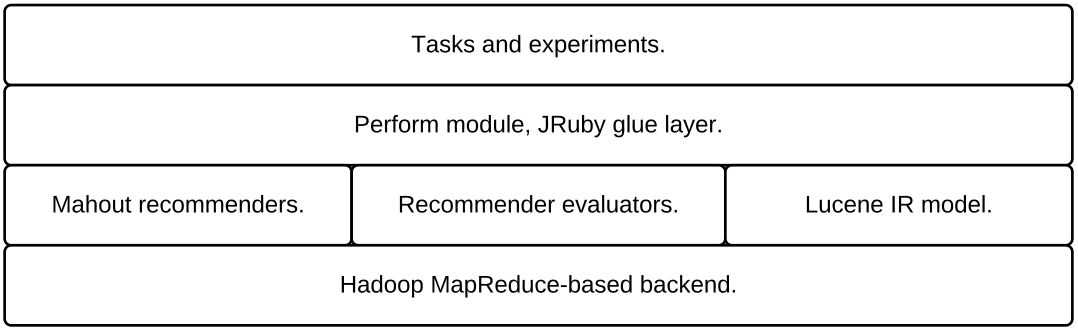
\includegraphics[
      width=1.0\textwidth]{../graphics/diagram-app-layers}
    \caption[Library Layers]{
      Library layers:
      Tasks and experiments are performed by the custom JRuby glue layer.
      Recommenders are created by the Mahout machine learning library.
      IR models are based on the Lucene search engine library.
      Recommender evaluators are created in Ruby.
      Each of the intermediary layers are built on the Hadoop
      MapReduce framework for efficient parallel computation. 
    }
  \label{fig:library-layers}
  \end{center}
\end{figure}

Naturally, the most important part of the implementations are the recommender systems.
These are used for the basic ratings predictions, and to 
create the adaptive aggregation by predicting the accuracy of other recommenders.
At the same time, these different recommenders need to have the same
interface for training and testing, regardless of which context
each experiment places them into.
Our implementation makes use of a number of external libraries,
as seen in Figure \ref{fig:library-layers}

To quickly get a large number of recommenders up and running,
the system was linked with the \emph{Apache Mahout machine learning library}
(See Appendix \ref{appendix:resources}). 
Mahout provides a number of machine learning
algorithms, amongst which a set of recommender systems.
Examples include SVD- and KNN-based recommenders,
baseline recommenders, a Slope One recommender,
cluster-based recommenders,
and various generic recommenders for mixing different 
similarity and neighborhood measures.
Mahout is a young project, launched in 2008, 
but was found to be quite mature and feature-rich
in our experience.

Mahout is build on top of \emph{Apache Hadoop},
a system for creating scalable and distributed data processing systems 
(See Appendix \ref{appendix:resources}).
This is important to the performance of our system.
As mentioned, a lot of the operations performed in layering recommenders
are independent and lend themselves well to parallelization.
By building on Hadoop, each of our recommenders come implemented in a 
proper MapReduce framework for parallel computation (as explained in \citet[p75]{Manning2008}).
Each of the basic recommenders and adaptive aggregators can then be modeled at the same time,
making the most out of whatever hardware is present.

For our IR tasks, we chose to build on another library.
\emph{Apache Lucene} (See Appendix \ref{appendix:resources}) is an open-source search engine, also built on top of Hadoop,
gaining the same performance wins as Mahout.
Lucene provides powerful methods for creating indexes of items, and for querying these indexes.

Mahout, Lucene and Hadoop are all written in the Java Programming Language,
and runs on the Java Virtual Machine (JVM).
To facilitate rapid prototyping, the Ruby scripting language was chosen as a "glue" language,
for interfacing with the libraries. 
By using the JRuby implementation of Ruby, Java libraries can be imported directly
into the language, allowing us to use Mahout and Hadoop almost as if they were written in the same language.
The use of Ruby allowed us to quickly develop different combinations of recommenders and
perform varying experiments in a short amount of time.

\section{Task Structure}

\begin{figure}[t]
  \begin{center}
    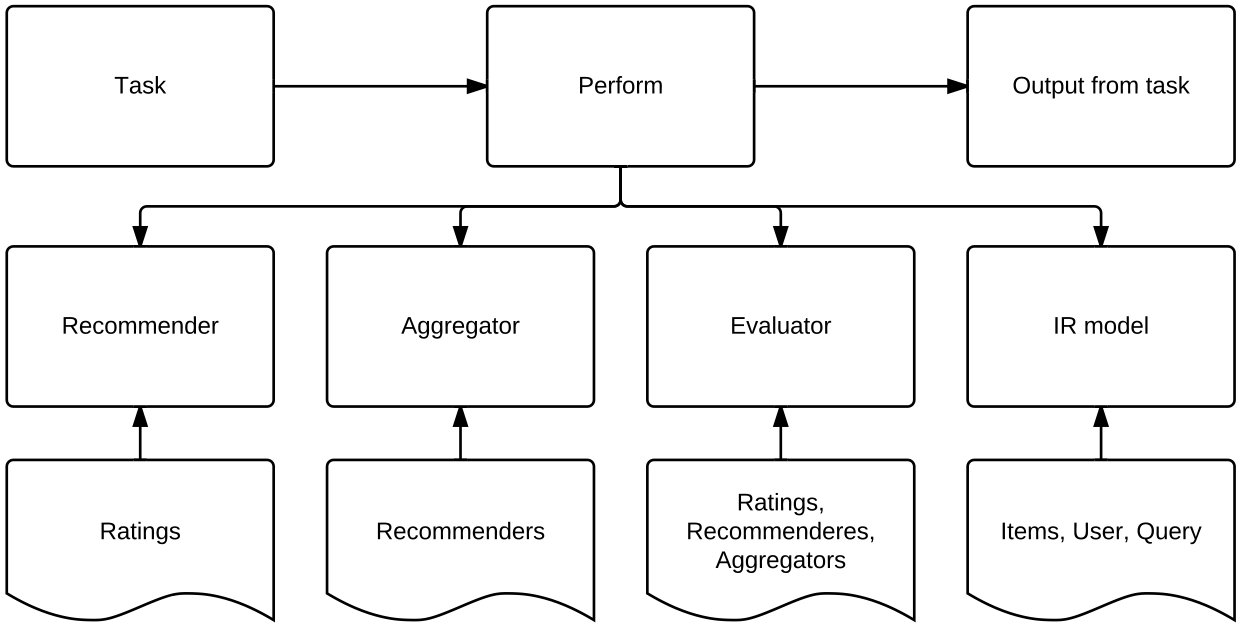
\includegraphics[
      width=1.0\textwidth]{../graphics/diagram-task}
    \caption[Task Structure Diagram]{
      Task structure diagram:
      A task (instantiated config) is passed to the perform module.
      This module creates a number of modules:
      recommenders, aggregators, evaluators and information retrieval models.
      Each module takes a set of inputs (bottom row), 
      which are specificed by the current task.
      These modules are then used as needed by each experiment.
    }
  \label{fig:uml}
  \end{center}
\end{figure}

In order to facilitate rapid prototyping,
our system is built around a few core concepts that can
be used together in different ways.
Everything the system does is considered a \emph{task}.
A task is a collection of settings and directives
and serves as instantiated configurations for the system.
Tasks are created beforehand, and fed into the sytem,
which carries them out.
Tasks specify what the system should do,
which dataset should be used, and other options.
See Figure \ref{fig:uml} for the overall structure.

The most important task is creating a recommender.
As recommenders are used both for the standard rating predictions,
and for the adaptive error estimations, creating recommenders
are the most common and important task of this system.
Another important task is creating evaluators.
An evaluator takes a set of recommenders as input,
tests them against the dataset specified in the task,
and returns the results of the evaluation.


\section{Modeling \emph{\&} Prediction}

The modeling phase consists of running our modeling algorithms and storing the resulting models.
A task is created for each of the basic recommenders, and for each of the adaptive recommenders.
If this is a rank aggregation scenario, an IR model is also created, based on the data
specified by the current task.
As mentioned, this is an offline approach, so that the models can be computed and recomputed,
indepentent of making any actual predictions.

Our experiments required us to measure the performance of each
recommender, and the adaptive recommender, for every combination of 
a user and an item.
In order to perform these experiments, an \emph{evaluator} module was built.
As both the standard recommenders and the adaptive recommender system presents the same 
interface, the evaluators simply takes a set of recommenders as input, 
and measures their accuracy across the dataset specified by the current task.

This prediction phase, where each user is compared to every un-rated item,
is not comparable to the prediction phase of a real-world system
based on adaptive recommenders. In a real world application of this technique,
a prediction is made whenever a user's actions requires it,
e.g. when we need to know what a user will think of an item.

This is where the $\mathrm{MapReduce}$ operations previously mentioned come into play.
Each of the basic recommenders, and each of the adaptive recommenders can be applied in parallel.
The basic recommenders are applied through a $\mathrm{map}$ operation, where the current user and item (the input)
is given to each modeling method. These methods return a number of scalar predictions.
The next step is the $\mathrm{reduce}$ operation, which is the adaptive layer.
Here, the scalar predictions are reduced to one prediction by computing weights
based on probable accuracy.
These computations can of course be cached, if certain combinations of users and items
often need predictions.

As mentioned, none of these aspects have any bearing on the viability of adaptive recommenders.
However, as this does provide an example of how to implement such a system. 
See Appendix \ref{appendix:resources} for links to other resources. 



\chapter{Resources}
\label{appendix:resources}

This appendix gives pointers to additional resources mentioned throughout this thesis.

\section{Implementation Code}

The code for the implementation outlined in Appendix \ref{appendix:implementation} is available online.
It resides in version control at 
\url{github.com/olav/thesis/tree/master/code}.

The implementation is built on three open-source libraries from the
Apache Project\footnote{See \url{www.apache.org/} --- accessed 19/5/2011}:
The Hadoop distributed computing library\footnote{See \url{hadoop.apache.org/} --- accessed 19/5/2011},
the Mahout machine learning library\footnote{See \url{mahout.apache.org/} --- accessed 19/5/2011},
and the Lucene information retrieval library\footnote{See \url{lucene.apache.org/} --- accessed 19/5/2011}.

Specific versions of these libraries are bundled together with
the source code as JAR-files, that run on the JVM.
Note that these libraries are released under their own terms,
namely the Apache License\footnote{
See \url{www.apache.org/licenses/} --- accessed 19/5/2011}.
The repository also includes the glue-code, written in ruby and run on the JRuby\footnote{
See \url{www.jruby.org/} --- accessed 09/05/2011} interpreter.

\section{Document Details}

This thesis is written in the LaTeX document preparation system.
It is based on a LaTeX-template called Memoir\footnote{
See \url{www.ctan.org/tex-archive/macros/latex/contrib/memoir/} --- accessed 19/5/2011.}.
Most of the figures and graphs are made with the TikZ and PGF graphics libraries\footnote{
See \url{www.texample.net/tikz/} --- accessed 23.05.2011}.

The entire source code for this document can be found at 
\url{github.com/olav/thesis/tree/master/thesis}.
The most current PDF-version is also available from this site.
%The source code for the implentation, this document, and the thesis itself
%is available under a Creative Commons BY 3.0 license\footnote{
%See \url{creativecommons.org/licenses/by/3.0/}}.
%Anyone is free to share, copy, distribute or transmit this work,
%or adapt it for any purpose,
%as long as the work is attributed to its author.
For citation purposes, use the following BibTex entry:

{
\footnotesize
\begin{verbatim}
@mastersthesis{Bjørkøy2011,
  address = {Trondheim, Norway},
  author  = {Bjørkøy, Olav},
  school  = {NTNU},
  year    = {2011},
  title   = {{Adaptive Recommenders: 
              Personalized Prediction Aggregation
              Through Accuracy Estimation}}
} 
\end{verbatim}
}


    \end{appendices}

  \backmatter
    {
  %\footnotesize

  \bibliographystyle{apalike}      

  \bibliography{library}
}

    
\end{document}

